\documentclass[a4paper,12pt]{wihuri}
%\usepackage{isolatin1} % Saadaan ��kk�set toimimaan !
%\usepackage[latin1]{inputenc} % Saadaan oikeat merkit
\usepackage[utf8]{inputenc} % T�ll� toimii utf-8
\usepackage[T1]{fontenc}      % Ja t�m� liittyy edelliseen
\usepackage[english]{babel} %Suomenkielinen tavutus
\usepackage{tytiivis} %Tiivistelm�sivun laatimiseksi
\usepackage{tytiivis2}
\usepackage[pdftex]{graphicx}%Saadaan kuvat toimimaan
\usepackage{pdfpages}
\usepackage{float}
\usepackage{amsmath}
\usepackage{amsfonts}
\usepackage{amssymb}
\usepackage{amsthm}							%identity operator \mathbb{1}
\usepackage{lastpage}
\usepackage{array}
\usepackage{braket}
\usepackage{dsfont}
\usepackage[shortlabels]{enumitem}
\inputencoding{utf8} %encoding for äö in bibliography


%%%%%%%%%%%%%%%%%%%%%%%%%%%%%%%%%%%%%%%%%%%%%%%%%%%%%%%%
%----- THEOREM STYLES
%%%%%%%%%%%%%%%%%%%%%%%%%%%%%%%%%%%%%%%%%%%%%%%%%%%%%%%%
\theoremstyle{definition}
\newtheorem{definition}{Definition}
\newtheorem{example}{Example}
\newtheorem{theorem}{Theorem}
\newtheorem{proposition}{Proposition}
\newtheorem{lemma}{Lemma}

%%%%%%%%%%%%%%%%%%%%%%%%%%%%%%%%%%%%%%%%%%%%%%%%%%%%%%%%
%----- THEOREM LABELING
%%%%%%%%%%%%%%%%%%%%%%%%%%%%%%%%%%%%%%%%%%%%%%%%%%%%%%%%
\numberwithin{definition}{section}
\numberwithin{example}{section}
\numberwithin{theorem}{section}
\numberwithin{proposition}{section}
\numberwithin{lemma}{section}

%%%%%%%%%%%%%%%%%%%%%%%%%%%%%%%%%%%%%%%%%%%%%%%%%%%%%%%%
%----- CUSTOM COMMANDS
%%%%%%%%%%%%%%%%%%%%%%%%%%%%%%%%%%%%%%%%%%%%%%%%%%%%%%%%
\newcommand{\I}{\mathcal{I}}%Instrumentti I
\newcommand{\ins}{\I_X^{\mm}}%I Schrödingerin kuvassa
\newcommand{\insd}{\I_X^{\mm *}}%I Heisenbergin kuvassa
\newcommand{\hi}{\mathcal{H}}%Hilbert
\newcommand{\ki}{\mathcal{K}}%2. Hilbert
\newcommand{\N}{\mathcal{N}}%Hilbert subspace
\newcommand{\salg}{\mathcal{F}}%sigma-algebra

\newcommand{\lin}{\mathcal{L}}%Lineaarioperaattori
\newcommand{\tc}{\mathcal{T}}%Trace-class
\newcommand{\tila}{\mathcal{S}}%Tila
\newcommand{\effect}{\mathcal{E}}%Efektit
\newcommand{\selfadj}{\mathcal{L}_{s}}%Itseadjungoituvat
\newcommand{\projection}{\mathcal{P}}%Projektiot
\newcommand{\unitary}{\mathcal{U}}
\newcommand{\EC}{\mathcal{E}}

\newcommand{\borel}{\mathfrak{B}}


\newcommand{\J}{\text{poislukien Juho}}
\newcommand{\mm}{\mathcal{M}}%Mittausmalli
\newcommand{\V}{\mathcal{V}}%Kanava V
\newcommand{\A}{\mathsf{A}}%Suure A
\newcommand{\B}{\mathsf{B}}%Suure B
\newcommand{\C}{\mathsf{C}}%Suure C
\newcommand{\F}{\mathsf{F}}%Suure F
\newcommand{\M}{\mathsf{M}}%Suure M
\newcommand{\E}{\mathsf{E}}%Suure E
\newcommand{\p}{\mathsf{P}}%Suure P
\newcommand{\Q}{\mathsf{Q}}%Canonical Position Observable

\newcommand{\id}{\mathds{1}}
\newcommand{\cc}{\mathbb{C}^2}%dim 2 C 
\newcommand{\real}{\mathbb{R}}%Real numbers
\newcommand{\nat}{\mathbb{N}}
\DeclareMathOperator{\tr}{tr}
\newcommand{\norm}[1]{\left\lVert#1\right\rVert}
%\newcommand{\tr}[1]{\left[\#1\right]}

\newcommand{\sat}{\mathfrak{s}}

\newcommand{\pp}{\preceq_{post}}
\newcommand{\spp}{\simeq_{post}}
\newcommand{\ppeq}{\prec_{post}}


\newenvironment{psmallmatrix}
  {\left(\begin{smallmatrix}}
  {\end{smallmatrix}\right)}


\begin{document}

\title{Sequential Quantum Measurements}%Title of the thesis
\opinnayte{Master's Thesis}
\author{B.Sc. Tuomas Tammero}
\vuosi{2018}
\oppiaine{Theoretical Physics}
\tarkastaja{Docent Teiko Heinosaari}
\tarkastaja{Prof. Sabrina Maniscalco}
\maketitle

%\newpage%This is the Turnitin page. This should be printed on the backside of the previous page.
%\thispagestyle{empty}
%\null
%\vfill

%\noindent The originality of this thesis has been checked in accordance with the University of Turku quality assurance system using the Turnitin OriginalityCheck service.

%\vspace{0.7cm}
%\noindent Turun yliopiston laatujärjestelmän mukaisesti tämän julkaisun alkuperäisyys on tarkastettu Turnitin OriginalityCheck -järjestelmällä.

\begin{tiivistelma}%Abstract
        {Department of Physics and Astronomy}%
        {TAMMERO, TUOMAS:}%Tekijän suku- ja etunimi
        {Sequential Quantum Measurements}%Tutkielman otsikko
        {Master's thesis, XX pages}% , YY appendix pages
        {Theoretical physics}% Oppiaine
        {November 2018}%tutkielman valmistumisvuosi ja -kuukausi

This thesis studies the field of quantum measurements and more precisely sequential measurements. The aim is to provide answers to questions like when is performing a sequential or a repeated measurement meaningful, or even possible. This is important in order to understand what type of information can be acquired when performing measurements on quantum states. 

In basic quantum theory observables are identified with self-adjoint operators. We introduce the concept of a positive operator valued measure (POVM) to gain better understanding on observables. The downside to POVMs is that they don't produce a new state after the measurement, only measurement statistics. In order to perform multiple measurements on a quantum state, the concepts of measurement model and instrument are defined in this thesis. Using instruments to perform measurements is essential in order to describe a state after the initial measurement is performed. This way it's possible to make measurements sequentially.

After defining the necessary tools for sequential measurements and a few different properties related to them, some applicable situations for these kind of measurements are shown. This way sequential measurements end up being somewhat meaningful in order to gain information from quantum systems.




\noindent Keywords: Measurement, Sequential Measurement, Observable, Measurement Model, Instrument
\end{tiivistelma}


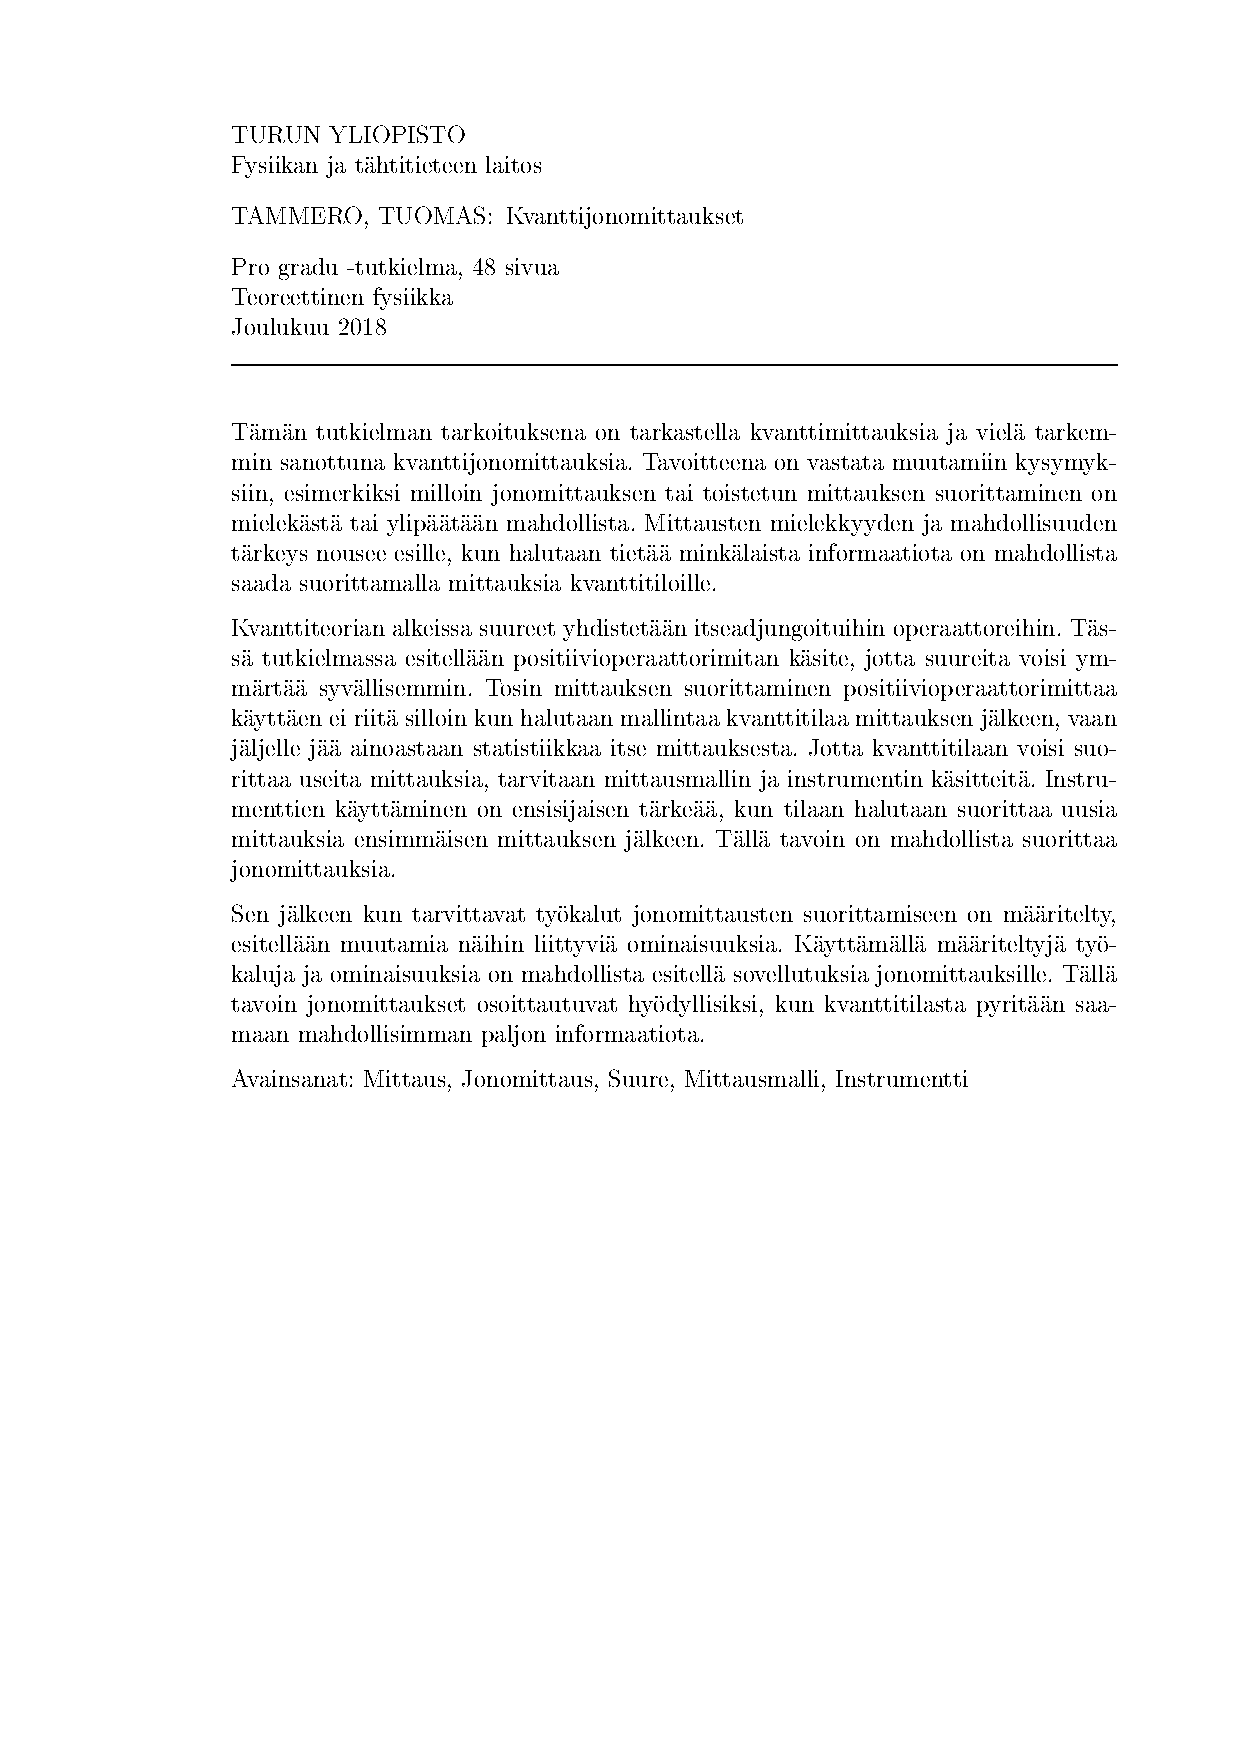
\includepdf[pages=-, offset=2.55cm -2.55cm]{tiivistelma.pdf}
	


\tableofcontents %Sis�llysluettelo
\newpage
\section*{Introduction}
\thispagestyle{empty}
\addcontentsline{toc}{section}{Introduction}
Measurements in the quantum world are extremely different from what they are in the classical sense. Classically, it's possible to measure almost anything with precision, given the limitations of our measurement devices. As an example a classical system containing only a single particle is fully described by it's location and momentum, both of which can be measured. In quantum theory, states are used to describe the system and a measurement is performed directly on the state. These measurements performed on states often disrupt the state in one way or another. We might not be able to perform another measurement to a state after an initial measurement is made or the measurement itself could alter the state somehow. 

The objective of this thesis is to showcase and study a variety of measurement setups, which affect the measured state in different ways. Starting from the rudiments of quantum mechanical framework and the most basic notion of an observable, a positive operator valued measure, we work our way to measurement models and instruments. The aim is to introduce the necessary tools needed to perform multiple measurements in the initial state, which is essentially what sequential measurements mean. A special case of sequential measurement is repeatable measurements, where a measurement of a single observable is performed multiple times. We study how measuring observables sequentially alter the quantum state in each step and when performing these types of measurements is meaningful.

Quantum measurements have a variety of features which are introduced in this thesis. For example the notion of non-disturbance, which shows what kind of measurements can be performed without disturbing the initial state. Another feature closely related to non-disturbance worth mentioning is joint measurability, where we'll study what kind of observables can be measured jointly on the quantum state. 

In the final chapter we'll go through some applicable scenarios where a sequential measurement can be performed, including the canonical position observable. The point is to show that after thoroughly showcasing quantum measurements and the related properties, the studied measurement setups are in fact useful when studying real quantum systems.

\newpage

\section{Quantum Mechanical Framework}
%references:\cite{busch_lahti_cassinelli_foundations}\cite{heinosaari_wolf_nondisturbance}\cite{heinosaari_miyadera_universality}\cite{Ozawa}\cite{heinosaari_ziman_2011_book}\cite{hamamura_miyadera_statedistinction}\cite{busch_spin_joint}\cite{heinosaari_notes_on_joint}\cite{heinosaari_simultaneous}\cite{saturation}\cite{intristic_unsharpness}\cite{kuramochi_constrution} \cite{Tumulka2008_kolmogorov}\cite{paulsen_vern}\cite{reed_simon_math_physics}\cite{davies1970} \cite{rudin}\cite{MQP}\cite{luders}

In this chapter, all the important bits and pieces of quantum theory needed to understand this work are presented with examples. The source of these important definitions is the book\cite{heinosaari_ziman_2011_book}. While the book is extremely comprehensive, only the most important parts needed to present quantum measurements and more precisely, sequential measurements, are reviewed here.

\subsection{Hilbert spaces}
The most fundamental mathematical concept in quantum theory is that of Hilbert space. While the definition itself in not too complex, it's important to recall what is meant by Hilbert space, since they are needed throughout this thesis. We'll start off by defining an inner product in a complex vector space.
\begin{definition}
Let $\hi$ be a complex vector space. The function $\braket{\cdot | \cdot}$ on $\hi \times \hi$ is called an inner product if,
\begin{enumerate}[i)]
\item $\braket{\varphi | c\psi + \phi} = c\braket{\varphi | \psi} + \braket{\varphi | \phi} , \quad \forall c \in \mathbb{C},\quad \varphi, \psi, \phi \in \hi$
\item $\overline{\braket{\varphi | \psi}} = \braket{\psi | \varphi}$
\item $\braket{\varphi | \varphi} > 0, \quad $ if $\varphi \neq 0$
\end{enumerate}

%--------- DEFINITION: CAUCHY SEQUENCE ---------------------

\end{definition}
Inner product defines a norm $\norm{\varphi} := \sqrt{\braket{\varphi | \varphi}}$  in $\hi$, making $\hi$ a normed space. Moreover, a metric $d(\cdot,\cdot)$ can be defined using this norm, $d(\varphi, \psi) = \norm{\varphi - \psi}$, which leads to the definition of a complete metric space\cite{heinosaari_ziman_2011_book}.
\begin{definition}
Let $\lbrace \varphi_i \rbrace$ be a sequence in $\hi$. The sequence is called a Cauchy-sequence, if for every $\varepsilon > 0$, there exists $N_{\varepsilon} \in \mathbb{N}, N_\varepsilon > 0$ such that $d(\varphi_i, \varphi_j) < \varepsilon$ when $i,j > N_{\epsilon}$. A metric space $\hi$ is said to be complete, if every Cauchy-sequence in $\hi$ converges. 
\end{definition}

\begin{example}

\end{example}
Let $\varphi_i = \frac{1}{2^i}$ and $\varepsilon > 0$. Then choose $N_\varepsilon > 0$ so that $\frac{1}{2^{N_\varepsilon}} > \varepsilon$, $\frac{2}{2^{N_\varepsilon}} = \varepsilon$ and $i,j > N_\varepsilon$ which leads to
\begin{align*}
d(\varphi_i, \varphi_j) &= \norm{\dfrac{1}{2^i} - \dfrac{1}{2^j}} \leq \dfrac{1}{2^i} + \dfrac{1}{2^j} \\
&\leq \dfrac{1}{2^{N_\varepsilon}} + \dfrac{1}{2^{N_\varepsilon}} = \varepsilon,
\end{align*}
which proves that $\{ \varphi_i \}$ is Cauchy.

To show an example of a sequence, which is not Cauchy, let $\varphi_i = \ln i$. From this we get
\begin{align*}
d(\varphi_{i+1}, \varphi_{i}) &= \norm{\ln(i+1) - \ln i} = \ln(1+\dfrac{1}{i}) \\
&\rightarrow \ln 1 = 0\text,
\end{align*}
from which it's clear that the sequence is not Cauchy.

Combining the already defined inner product and completeness leads to the following definition.
\begin{definition}
A inner product space, which is complete, is called a Hilbert space.
\end{definition}


From now on $\hi$ always denotes a complex and separable Hilbert space, meaning a Hilbert space with a countable orthonormal basis. 
%The outcomes of observables in $\hi$ are represented using the outcome set $\Omega$ and the $\sigma$-algebra of this set, $\salg$. 
Though there are a number of interesting Hilbert spaces to consider, we'll mostly focus on the two-dimensional complex space, $\hi = \cc$.

\subsection{Hilbert Space Operators}
There are multiple important sets of operators with a variety of different attributes, all necessary to define for their own purposes. But first, we need the very basic definition of a bounded operator. 


%---------- DEFINITION: BOUNDED OPERATOR ---------------------
\begin{definition}
Let $T:\hi \rightarrow\hi$ be a linear mapping. $T$ is a bounded operator if there is a $t \geq 0$, for which
\begin{align*}
\norm{T\psi} \leq t\norm{\psi}, \quad \forall \psi \in \hi \text.
\end{align*} 
The set of bounded operators is denoted with $\lin(\hi)$. Moreover, each bounded operator $T$ has an adjoint operator $T^*$ defined by 
\begin{align*}
\braket{\varphi|T^* \psi} = \braket{T\varphi|\psi}.
\end{align*}
Using the adjoint operator, the absolute value of operator can also be defined as
\begin{align*}
|T| = (T^*T)^{1/2}\text.
\end{align*} 
\end{definition}


The following sets of bounded linear operators are used throughout this thesis and form an integral part of quantum theory.
\begin{enumerate}[$\bullet$]
\item The set of selfadjoint operators, $\selfadj(\hi)$. A linear operator $L$ if selfadjoint, if $L = L^*$.
\item The set of projections, $\projection(\hi)$. A selfadjoint operator $P$ is a projection, if $P^2=P$.
\item The set of unitary operators, $\unitary(\hi)$. A bounded operator $U$ is unitary if $U^*U = UU^* = \id$.
\item The set of trace class operators, $\tc(\hi)$. A bounded operator $T$ is trace class if $\tr[|T|] < \infty$.
\item The set of states, $\tila(\hi)$. A trace class operator $\rho$ is a state, if it's positive and of trace one. The state $\rho$ is pure, if it's also a one-dimensional projection.
\item The set of effects, $\effect(\hi)$. A selfadjoint operator $E$ is an effect, if $O \leq E \leq \id$.
\end{enumerate}
\begin{example}
We'll show some examples of these kind of operators in the Hilbert space $\cc$.

\begin{enumerate}[$\bullet$]
\item An example of a selfadjoint operator in $\cc$ would be any real valued 2x2 matrix.
\item An example of a projection in $\cc$ is the matrix 
$P=\begin{pmatrix}
0 & 0 \\
0 & 1
\end{pmatrix}$, since clearly $P^2 = P$.
\item An example of a unitary operator in $\cc$ is a diagonal matrix 

$U = \begin{pmatrix}
ie^{-ix}& 0 \\
0 & ie^{-iy}
\end{pmatrix},\quad$ where $x,y \in \real$.
\item An example of a trace class operator in $\cc$ is any real or complex valued 2x2 matrix.
\end{enumerate}
\end{example}


When working with sequences of operators and their convergence, the convergence is referred as weak or strong. This means that the convergence happens with respect to either the weak or strong operator topology.

%------ OPERATOR TOPOLOGIES COMMENTED OUT, USE DEFINITIONS OF CONVERGENCE INSTEAD FOR SIMPLICITY
\begin{definition}
Let $\{ T_i\}$ be a sequence of bounded operators, $T_i \in \lin(\hi)$ for every index $i$. 
\begin{enumerate}[a)]
\item The sequence converges strongly to an operator $T \in \lin(\hi)$ if $\lim T_i \varphi = T\varphi,\, \forall \varphi \in \hi$.
\item The sequence converges weakly to an operator $T \in \lin(\hi)$ if $\lim \braket{\varphi | T_i \psi} = \braket{\varphi | T\psi},\, \forall \varphi,\psi \in \hi$.
\end{enumerate}
\end{definition}

Throughout this thesis convergence is always referred to be either strong or weak and by the above definition, the convergence can be thought to happen with respect to either the norm or inner product.
%--------- EXAMPLE OF STRONG CONVERGENCE
%\begin{example}


%\end{example}

%--------- EXAMPLE OF WEAK CONVERGENCE



%------------ STRONG OPEARTOR TOPOLOGY --------

%\begin{definition}
%The strong operator topology is defined to be the weakest topology on $\lin(\hi)$ for which the maps
%\begin{align*}
%E_\varphi : \lin(\hi) \rightarrow \hi \\
%E_\varphi(T) = T\varphi
%\end{align*}
%are continuous $\forall \varphi \in \hi$. A basis is given by sets with the following form
%\begin{align*}
%\{S\, |\, S \in \lin(\hi), \quad \norm{S\varphi_i}_\hi < \varepsilon, \quad i = 1,\,\ldots,n \}
%\end{align*}
%where $\{ x_i\}_{i=1}^n$ are elements in $\hi$ and $\varepsilon > 0$. In the strong operator topology a net of operators $\{ T_j\}$ converges to an operator $T$ if and only if
%\begin{align*}
%\norm{T_j\varphi - T\varphi}\rightarrow 0,\quad \forall \varphi \in \hi\text.
%\end{align*}
%This kind of convergence is also called strong convergence.
%\end{definition}%%

%------------- WEAK OPERATOR TOPOLOGY

%\begin{definition}
%The weak operator topology is defined as the weakest topology on $\lin(\hi)$ such that the maps
%\begin{align*}
%&E_{\varphi, l} : \lin(\hi, \hi^*) \rightarrow \mathbb{C},\\
%&E_{\varphi, l}(T) = l(T\varphi)
%\end{align*}
%are continuous $\forall \varphi \in \hi,\,l\in\hi^*$. A basis is given by sets with the following form
%\begin{align*}
%\{S\,|\,S \in \lin(\hi, \hi^*),\quad |l_i(T\varphi_j)| < \varepsilon , \quad i = 1,\,\ldots,n,\,j=1,\,\ldots,m \}
%\end{align*}
%where both $\{ x_1\}_{i=1}^n \in \hi$ and $\{l_j \}_{j=1}^m \in \hi^*$ are finite. In the weak operator topology a net of operators $\{ T_k \}$ converges to an operator $T$ if and only if
%\begin{align*}
%|l(T_k\varphi) - l(T\varphi)| \rightarrow 0, \quad \forall l \in \hi^*, \varphi \in \hi\text.
%\end{align*}
%This kind of convergence is also called weak convergence.
%\end{definition}

%In simpler terms, a net of operator $\{ T_k \}$ converges strongly to an operator $T$, if $\lim T_k \varphi = T \varphi, \, \forall \varphi \in \hi$. If the net $\{ T_k \}$ converges weakly, then $\lim \braket{\varphi | T_k \psi} = \braket{\varphi | T \psi},\,\forall \varphi, \psi \in \hi$.

Next up we will prove two closely related theorems, the Hilbert projection theorem and Riezs's lemma, both of which will later be needed when proving the Kolmogorov extension theorem for POVMs.

%----------- THE HILBERT PROJECTION THEOREM -------------
\begin{theorem}[The Hilbert Projection Theorem]
Let $\hi$ be a Hilbert space with a closed subspace $\N$. Every $\psi \in \hi$ can bee written as $\psi = \phi + \zeta$ where $\phi \in \N$ and $\zeta\in \N^\perp$. 

\noindent \textit{Proof} First we need to show that for $\psi \in \hi$ there exists a unique element $\phi\in\N$, which is closest to $\psi$. Let $d = \inf_{\varphi\in \N}\norm{\psi-\varphi}$ and let $\{\varphi_n\}$ be a sequence in $\N$ for which
\begin{align*}
\norm{\psi -\varphi_n}\rightarrow d\text.
\end{align*}
It follows that
\begin{align*}
\norm{\varphi_n - \varphi_m}^2 &=\norm{(\varphi_n) - (\varphi_m)}^2 \\
&= 2\norm{\varphi_n-\psi}^2 + 2\norm{\varphi_m-\psi}^2 - \norm{-2\psi + \varphi_n + \varphi_m}^2 \\
&= 2\norm{\varphi_n-\psi}^2 + 2\norm{\varphi_m-\psi}^2 - 4\norm{\psi- \frac{1}{2}(\varphi_n+\varphi_m)}^2 \\
&\leq 2\norm{\varphi_n-\psi}^2 + 2\norm{\varphi_m-\psi}^2 - 4d^2 \\
&\rightarrow 2d^2 + 2d^2 - 4d^2 = 0,
\end{align*}
when $n \rightarrow \infty$ and $m \rightarrow \infty$. We can see that $\{\varphi_n\}$ is a Cauchy sequence and it converges to an element $\phi \in \N$ and $\norm{\psi - \phi} = d$. The element $\phi$ is also unique, since if there was another element $\phi'$ for which $\norm{\psi-\phi'} = d$ 
\begin{align*}
&\norm{\psi - \phi} = \norm{\psi - \phi'} \\
\Leftrightarrow &\norm{\psi - \phi}^2 = \norm{\psi - \phi'}^2 \\
\Leftrightarrow &\braket{\psi-\phi | \psi-\phi} - \braket{\psi-\phi' | \psi - \phi'} = 0 \\
\Leftrightarrow &\braket{\phi' - \phi | \phi' - \phi} = 0 \\
\Leftrightarrow &\, \phi' = \phi \text.
\end{align*}
Now with $\phi$ being the element closest to $\psi$ we can define $\zeta = \psi - \phi \Leftrightarrow \psi = \phi + \zeta$. Let $\varphi \in \N$ and $\alpha \in \real$. For $d = \norm{\psi - \phi}$ we have
\begin{align*}
d^2 &\leq \norm{\psi - (\phi + \alpha\varphi)}^2 = \norm{\zeta - \alpha\varphi}^2 \\
&= d^2 - 2\alpha\cdot\text{Re}(\braket{\zeta|\varphi}) + \alpha^2\norm{\varphi}^2 \\
\Rightarrow& -2\alpha\cdot\text{Re}(\braket{\zeta|\varphi}) + \alpha^2\norm{\varphi}^2 \geq 0,
\end{align*}
from which we get Re$(\braket{\zeta|\varphi})=0$. Similarly, by using $i\alpha \in \mathbb{C}$ instead of the real scalar we get Im$(\braket{\zeta|\varphi})=0$ and it follows that $\zeta \in \N^\perp$. Furthermore $\zeta$ is unique, since if there were another $\zeta'$ for which $\psi = \phi + \zeta = \phi + \zeta'$, we get
\begin{align*}
&\norm{\zeta - \alpha\varphi}^2 = \norm{\zeta' - \alpha\varphi}^2\\
\Leftrightarrow & \braket{\zeta - \alpha\varphi | \zeta - \alpha\varphi} = \braket{\zeta' - \alpha\varphi | \zeta' - \alpha\varphi} \\
\Leftrightarrow & \braket{\zeta' - \zeta | \zeta' - \zeta} = 0 \\
\Leftrightarrow &\, \zeta' = \zeta\text.
\end{align*}
\end{theorem}

%------------ RIESZ'S LEMMA ---------------------------


\begin{theorem}[Riesz's lemma]
For every functional $T:\hi \rightarrow \mathbb{C}$ there exists a unique $\psi_T \in \hi$ such that 
\begin{align*}
&T\varphi = \braket{\psi_T | \varphi} \quad \forall \varphi \in \hi,\\
&\norm{\psi_T}_\hi = \norm{T}_{\hi^*}\text.
\end{align*}
\textit{Proof} Let $\N$ be the set of vectors $\varphi \in \hi$ which $T\varphi = 0$. The continuity of $T$ guarantees that the subspace $\N$ of $\hi$ is closed. If $\N = \hi$ then it would follow that $T\varphi =\braket{0,\varphi} = 0, \, \forall \varphi\in \hi$, which completes the proof for $\N = \hi$. Assume that $\N \neq \hi$, then by the projection theorem\cite{reed_simon_math_physics} there exists a nonzero vector $\varphi_0 \in \N^\perp$ and we define
\begin{align*}
\psi_T = T^*\varphi_0\norm{\varphi_0}^{-2}\varphi_0,
\end{align*} 
which we will show to have the correct properties. Firstly, for $\varphi \in \N$ it's clear that $T\varphi = 0 = \braket{\psi_T| \varphi}$. If $\varphi = \alpha\varphi_0$ for some scalar $\alpha$ then
\begin{align*}
T\varphi = T\alpha\varphi_0 = \alpha T\varphi_0 = \braket{T^*\varphi_0\norm{\varphi_0}^{-2}\varphi_0 | \alpha\varphi_0} = \braket{\psi_| \alpha\varphi_0}\text.
\end{align*}
From the linearity of functions $T$ and $\braket{\psi_T | \cdot}$ and the fact that both agree on $\N$ and $\varphi_0$, it follows that they must also agree on the space, which is spanned by $\N$ and $\varphi_0$. The vector space spanned by $\N$ and $\varphi_0$ is $\hi$, since every vector $\psi \in \hi$ can be written as
\begin{align*}
\psi = \left(\psi - \frac{T\psi}{T\varphi_0}\varphi_0 \right) + \frac{T\psi}{T\varphi_0}\varphi_0
\end{align*}
and so, $T\varphi = \braket{\psi_T, \varphi},\, \forall \varphi \in \hi$. If there exists another vector $\psi'\in\hi$ for which $T\varphi = \braket{\psi'|\varphi}$, then it follows that 
\begin{align*}
&\norm{\psi' - \psi_T}^2 = T(\psi' - \psi_T) - T(\psi' - \psi_T) = 0 \\
\Rightarrow& \psi' = \psi_T,
\end{align*}
which proves the uniqueness of $\psi_T$. Furthermore, the fact that $\norm{T}_{\lin(\hi)} = \norm{\psi_T}_\hi$ holds follows from
\begin{align*}
\norm{T} = \sup_{\norm{\varphi} \leq 1} |T\varphi| = \sup_{\norm{\varphi} \leq 1} |\braket{\psi_T,\varphi}| \leq \sup_{\norm{\varphi} \leq 1} \norm{\psi_T}\norm{\varphi} = \norm{\psi_T}
\end{align*}
and
\begin{align*}
\norm{T} = \sup_{\norm{\varphi} \leq 1} |T\varphi| \geq \left| T\left(\frac{y_T}{\norm{y_T}} \right) \right| = \braket{\psi_T | \psi_T / \norm{\psi_T}} = \norm{\psi_T},
\end{align*}
which completes the proof \cite{reed_simon_math_physics}.\hfill $\square$
\end{theorem}

Before introducing observables, we need to define a key feature for them, which is their spectral decomposition. Spectral decomposition often makes handling the math around observables much easier.
\begin{theorem}
For a trace class operator $T$, there exists an orthonormal basis $\lbrace \varphi_i \rbrace$ and a sequence of complex numbers $\lbrace \lambda_i \rbrace$ for which
\begin{align*}
T = \sum_i \lambda_i \ket{\varphi_i}\bra{\varphi_i}\text{.}
\end{align*}
For operators not in the trace class, a spectral decomposition exists, but the decomposition itself might have to be written as an integral instead of a sum.
\end{theorem}

\subsection{Observables}
Before any measurements can be performed, observables need to be defined. In introduction level quantum physics, observables are often presented as selfadjoint operators. For the purposes of this thesis, this representation of observables is not sufficient. Here observables are identified as positive operator valued measures (POVM's), which are mappings from a chosen $\sigma$-algebra $\salg$, to the set of effects in the Hilbert space, $\effect(\hi)$. 
%------------------------------------------------------------------------------------
%---------------- SIGMA ALGBRA ------------------------------------------------------
%-----------------------------------------------------------------------------------
\begin{definition}
A $\sigma$-algebra $\salg$ on a nonempty set $\Omega$ is a collection of subsets, which has the following three properties
\begin{enumerate}[i)]
\item $\emptyset \in \salg, \quad \Omega \in \salg$
\item $X \in \salg \Rightarrow \Omega \setminus X \in \salg$
\item $X_1, X_2, ... \in \salg \Rightarrow \cup_i X_i \in \salg$
\end{enumerate} 
\end{definition}
A measurable space is defined by the pair $(\Omega, \salg)$. Any set on the $\sigma$-algebra is called an event, which makes the $\sigma$-algebra a collection of events. By denoting $\borel(\Omega)$ we always denote the Borel $\sigma$-algebra of the set $\Omega$, which is defined as the smallest $\sigma$-algebra containing all the open sets of $\Omega$\cite{rudin}.
\begin{example}
Let's consider the set $\Omega = \lbrace 0, 1, 2 \rbrace$. The following collections of subsets are valid $\sigma$-algebras for the predefined set
\begin{enumerate}[$\bullet$]
\item $\lbrace \emptyset, \Omega\rbrace$
\item $\lbrace \emptyset, \Omega, 0, 1, 2, \lbrace 0,1\rbrace, \lbrace0,2\rbrace, \lbrace1,2\rbrace \rbrace$
\end{enumerate}

\end{example}
%---------------------------------------------------------------------
%------------------- POVM / OBSERVABLE --------------------------------
%-------------------------------------------------------------------------
With the $\sigma$-algebra defined, it's time to introduce the concept of a positive operator valued measure.
\begin{definition}
A POVM is a mapping $\A : \salg \rightarrow \effect(\hi)$, for which
\begin{enumerate}[i)]
\item $\A(\emptyset) = 0$
\item $\A(\Omega) = \id$
\item $\A(\cup_i X_i) = \sum_i \A(X_i)$, \quad with respect to the weak operator topology, for any sequence of disjoint sets $\lbrace X_i \rbrace \in \salg$
\end{enumerate}
\end{definition} 
\noindent Moreover, the mapping $\A$ is a POVM if and only if $X \mapsto \tr[\rho A(X)]$ represents a probability measure for all states $\rho \in \tila(\hi)$.


\begin{example}\label{qubitobs}
Let's consider the Hilbert space $\hi = \cc$. Now, any selfadjoint operator $A$ can be written using the operators $\id, \sigma_x, \sigma_y$ and $\sigma_z$ by composing a linear combination. This is a way to obtain a general effect on $\hi$,
\begin{align*}
A = \frac{1}{2}(\alpha \id + \vec{r}\cdot\vec{\sigma}), \quad \alpha \in \real, \vec{r} \in \real^3\text{.}
\end{align*}
The eigenvalues of $A$ are $\lambda_{\pm} = \frac{1}{2}(\alpha \pm \norm{\vec{r}})$. $A$ is in fact an effect if the following requirements are held
\begin{align*}
0 \leq \lambda_{-}, \quad \lambda_{+} \leq 1 \Rightarrow \norm{\vec{r}} \leq \alpha \leq 2 - \norm{\vec{r}}\text{.}
\end{align*}
\end{example}

This is the general definition of an observable. When an observable is said to be discrete, then $\A$ is a function, the outcome set $\Omega$ is finite and the sigma-algebra of the observable is just the power set of the outcome set $\Omega$. We use the notation $\A(X)$ when working with the general case and distinguish discrete observables using lowercase notation for the outcome, $\A(x)$. 
%---------------- PVM / SHARP OBSERVABLE -------------------------------

An important subset of POVMs are projection-valued measures, PVMs. PVMs are identified as sharp observables and have a little bit stricter definition than POVMs.
\begin{definition}
An observable $\A$ is sharp, if $\A(X)$ is a projection for every $X \in \salg$.
\end{definition}


\begin{example}
Let $\hi = \cc$. In $\hi$ sharp observables have only two possible outcomes, labelled here as $\pm 1$. Respectively, the corresponding operators $\A(-1)$ and $\A(1)$ are either $O$, $\id$ or some other one dimensional projection. If we exclude $O$ and $\id$, choose a vector $\vec{r} \in \mathbb{R}^3$, we can define
\begin{align*}
\A(-1) = \frac{1}{2}(\id - \vec{r}\cdot\vec{\sigma}), \quad \A(1) = \frac{1}{2}(\id + \vec{r}\cdot\vec{\sigma}),
\end{align*}
where $\vec{\sigma}$ denotes a vector with the Pauli matrices as elements. The corresponding selfadjoint operator for the observable $\A$ is 
\begin{align*}
A = \sum_i i\A(i) = \vec{r}\cdot \vec{\sigma}\text{.}
\end{align*}
\end{example}


%----------------- INFORMATIONALLY COMPLETE OBSERVABLES -----------------------

Observables can be characterized in multiple ways. One of these characterizations is informationally complete observables, which play an important role when discussing measurement features like non-disturbance and universality.
\begin{definition}
A collection of observables $\lbrace \A, \B, \ldots \rbrace$ is informationally complete, if for every pair of states the probability distributions of these observables being equal implies that the states are equal.

Often in literature a single observable $\A$ is said to be informationally complete instead of a set of observables. In this case, we require that the probability distribution of this observable being equal to every pair of states implies that the states are equal.
\end{definition}


%---------------- EXAMPLE: SIC POVM -------------------
\begin{example}
%As an example of a informationally complete observable, we'll use the simplest symmetric informationally complete observable or SIC-POVM for short\cite{sic_povm}. aaa
Let $\hi = \mathbb{C}^d$, of $\hi$ and let $P$ be a set of $d^2$ normalized vectors $\ket{\psi_k}$, for which
\begin{align*}
|\braket{\psi_k|\psi_j}|^2 = \dfrac{1}{d+1}, \quad k \neq j \text.
\end{align*}
The POVM elements corresponding to $P$ are the projections $\ket{\psi_k}\bra{\psi_k}/d = \Pi_k/d$. In order to have an informationally complete $P$, the operators $\Pi_k$ must be linearly independent, since they need to span the entire space of operators. To show linear independence we need to consider the rank of the Gram matrix of the operators. Using the previous equation we get
\begin{align*}
\tr[\Pi_j^*\Pi_k]  = \dfrac{d\delta_{jk} + 1}{d + 1}\text.
\end{align*} 



Due to the Kronecker delta and the constant value $d$, the Gram matrix here is circulant, meaning that each row is a cyclic shift of the previous. By definition the eigenvalue of each row is found using a Fourier transform to one of the rows and no eigenvalues are zero. This can be seen by choosing a complex number $\zeta\neq 1$ for which $\zeta^d = 1$, i.e. the $d$th root of unity defined by $\zeta=e^{2\pi i k/d}$ where $k = 1,\,\dots,d-1$, we can define a new orthonormal basis $\lbrace \varphi_i \rbrace$ using the set of vectors $\lbrace \psi_j \rbrace$ by
\begin{align*}
\varphi_i = \dfrac{1}{\sqrt{d+1}}\sum_{j=0}^d \zeta^{ij}\psi_j\text.
\end{align*}

Hence, the Gram matrix has a full rank, the projections $\Pi_k$ are linearly independent and $P$ is informationally complete\cite{sic_povm}.

\end{example}

%-------------------------- POST-PROCESSING ------------------------------

When it comes to sequential measurements, we need to define a pre-order of observables called post-processing. This gives us a way to compare two observables and the amount of information yielded from each.
\begin{definition}
Let $\A$ and $\B$ be observables with outcome sets $\Omega_\A$ and $\Omega_\B$, respectively. Denoting $\A \pp \B$ means that there exists a mapping $\kappa$, for which

\begin{align*}
&\kappa : \Omega_\A \times \Omega_\B \rightarrow [0,1]\\
\sum_x &\kappa(x,y) = 1, \quad \forall y \in \Omega_\B, \\
\A(x) = \sum_y &\kappa(x,y)\B(y), \quad \forall x \in \Omega_\A\text.
\end{align*}
A mapping $\kappa$ satisfying these conditions is called a Markov kernel, which form a convex set. Furthermore, denoting $\A \spp \B$ requires that both $\A \pp \B$ and $\B \pp \A$ hold. Denoting $\A \ppeq \B$ requires that $\A \pp \B$, but not $\B \pp \A$.

To show that post-processing really is a pre-order, we need to prove it's reflexivity and transitivity. Reflexivity follows straight from the definition of the mapping $\kappa$. For three observables $\A, \B, \C$, let $\A \pp \B$ and $\B \pp \C$, then
\begin{align*}
&\A(x) = \sum_y \kappa_1(x,y) \B(y), \quad \B(y) = \sum_Z \kappa_2(y,x) \C(z) \\
\Rightarrow & \A(x) = \sum_{y,z} \kappa_1(x,y)\kappa_2(y,z)\C(z)
\end{align*}
Since both $\sum_y \kappa_1(x,y) = 1$ and $\sum_Z \kappa_2(y,z) = 1$ and both $\kappa_1$ and $\kappa_2$ are mappings to the set $[0,1]$, post-processing is transitive and hence, a pre-order.
\end{definition}

%----------- EXAMPLE OF POST-PROCESSING ----------------
\begin{example}
Let $\A$ be a qubit observables of the form
\begin{align*}
\A(\pm 1) = \dfrac{1}{2}(\id \pm \vec{a}\cdot\vec{\sigma})\text. 
\end{align*}
To obtain another qubit observable $\B$, we need the applied post-processing $\kappa$ as
\begin{align*}
\kappa(+,+) = \kappa(-,-) &= s \\
\kappa(+,-) = \kappa(-,+) &= 1-s,\quad\text{ where }\,s\in \mathbb{C}\text.
\end{align*}
Using the above definition of post processing we get
\begin{align*}
\B(+1) &= \kappa(+,+)\A(+1) + \kappa(+,-)\A(-1) \\
&=\frac{1}{2}(s(\id + \vec{a}\cdot\vec{\sigma}) + (1-s)(\id - \vec{a}\cdot\vec{\sigma}))\\
&=\frac{1}{2}(\id + (2s-1)\vec{a}\cdot\vec{\sigma}),\\
\B(-1) &= \dfrac{1}{2}(\id - (2s-1)\vec{a}\cdot\vec{\sigma})\\
\Rightarrow \B(\pm 1) &= \frac{1}{2}(\id \pm (2s-1)\vec{a}\cdot\vec{\sigma})\text.
\end{align*}
So the chosen post-processing applied on the observable $\A$ yields an observable $\B$, which is almost the same as $\A$, but with the added noise factor $(2s-1)$. 


\end{example}

We defined post-processing for discrete observables, since this is what we'll use later in this thesis. In the definition of post processing for a general observable, the sum is replaced with an integral and $\kappa(\cdot, Y)$ is a probability measure and $\kappa(X, \cdot)$ is $\salg_\A$-measurable for every $X\in\salg_\A$.


%\begin{example}
%Let $\A$ and $\B$ be sharp two outcome qubit observables with outcomes $\A(\pm 1)$ and $\B(\pm 1)$. Post-processing can be achieved by using the Kronecker delta, i.e.
%\begin{align*}
%&\delta_{x, y} : \Omega_\A \times \Omega_\B \rightarrow [0,1],\\
%\sum_y &\delta_{x,y} = 1, \quad \forall y \in \Omega_\B \\
%\A(x) &= \sum_Y \delta_{x,y} \B(y), \quad \forall x \in \Omega_\A \\
%&= \B(x),
%\end{align*}
%which means that these two observables either give the same outcomes, or if $X \neq Y$ holds for every $Y$ the outcome statistics of these two observables %cannot be compared using post-processing.
%\end{example}

%------------------------------------------------------------------------------
%-------------- STINESPRING AND NAIMARK DILATION THEOREMS ---------------------
%------------------------------------------------------------------------------
\subsection{Dilation Theorems}
In this section we'll present two important and well-known dilation theorems, which are going to be very useful later in this thesis. The source of the proofs for these theorems is the book by Paulsen\cite{paulsen_vern}.

\begin{theorem}(Stinespring's dilation theorem)
Let $\EC^*: \lin(\hi) \rightarrow \lin(\hi)$ be a completely positive linear map. There exists another Hilbert space $\ki$, a unital *-homomorphism $\alpha : \lin(\hi) \rightarrow \lin(\ki)$ and a bounded operator $V: \hi \rightarrow \ki$ such that
\begin{equation}
\EC^*(T) = V^*\alpha(T)V, \quad \forall T \in \lin(\hi)\text{.}
\end{equation}
In addition if $V^*V = \id$ then $\EC^*$ is unital.
\end{theorem}
\noindent \textit{Proof} Let's define a symmetric bilinear function $\braket{\cdot|\cdot}$ in the tensor product $\lin(\hi) \otimes \hi$ by
\begin{align*}
\braket{T\otimes \varphi|L \otimes \psi} = \braket{\EC^*(L^*T)\varphi|\psi}_{\hi} 
\end{align*}
where $\braket{|}_{\hi}$ is the inner product in $\hi$. 

The function $\braket{|}$ is a positive semidefinite, which follows from the complete positivity of $\EC^*$, since
\begin{align*}
\left\langle\sum_{i=1}^n T_i \otimes \varphi_i|\sum_{j=1}^n T_j \otimes \varphi_j\right\rangle = \left\langle \EC_n^*(T_j^*T_i)\begin{psmallmatrix}
\varphi_1 \\
\vdots \\
\varphi_n
\end{psmallmatrix} | \begin{psmallmatrix}
\varphi_1 \\
\vdots \\
\varphi_n
\end{psmallmatrix} \right\rangle_{\hi^{(n)}} \geq 0,
\end{align*}
where $\braket{|}_{\hi^{(n)}}$ is the inner product in $\hi^{(n)}$, the direct sum containing the Hilbert space $\hi$ $n$ times. This inner product is defined by
\begin{align*}
\left\langle \begin{psmallmatrix}
\varphi_1\\
\vdots \\
\varphi_n
\end{psmallmatrix} \bigg| \begin{psmallmatrix}
\psi_1 \\
\vdots \\
\psi_n
\end{psmallmatrix} \right\rangle_{\hi^{(n)}} = \braket{\varphi_1 | \psi_1}_{\hi} + \cdots \braket{\varphi_n | \psi_n}_{\hi}\text{.} 
\end{align*}
Since every positive semidefinite bilinear function satisfies the Cauchy-Schwarz inequality, 
\begin{equation}\label{CS}
|\braket{\varphi | \psi}|^2 \leq \braket{\varphi | \varphi}\braket{\psi | \psi},
\end{equation}
we can define
\begin{align*}
\mathcal{N} &= \lbrace u \in \lin(\hi) | \braket{u | u} = 0 \rbrace \\
&=\lbrace u \in \lin(\hi) \otimes \hi | \braket{u | v} = 0, \, \forall v \in \lin(\hi) \otimes \hi \rbrace
\end{align*}
to be a subspace of $\lin(\hi) \otimes \hi$. The bilinear function on the newly defined quotient space $\lin(\hi) \otimes \hi / \mathcal{N}$
\begin{align*}
\braket{u + \mathcal{N} |v + \mathcal{N}} = \braket{u|v}
\end{align*}
is an inner product. Now let $\ki$ denote the Hilbert space, which is the completion of the quotient space $\lin(\hi) \otimes \hi / \mathcal{N}$ equipped with the inner product defined above.

For $T \in \lin(\hi)$, we'll define a linear map $\alpha(T) : \lin(\hi)\otimes\hi \rightarrow \lin(\hi)\otimes\hi$ by
\begin{align*}
\alpha(T)\left( \sum_i T_i \otimes \varphi_i \right) = \sum_i(TT_i)\otimes \varphi_i\text{.}
\end{align*}
From the factorization of the operator follows the inequality
\begin{align*}
T_i^*T^*TT_j \leq \norm{T^*T}(T_i^*T_j)
\end{align*}
and furthermore
\begin{align*}
&\left\langle \alpha(T)\left(\sum T_i \otimes \varphi_i\right), \alpha(T)\left(\sum T_j \otimes \varphi_j \right)\right\rangle \\
=&\sum_{i,j}\braket{\EC^*(T_j^*T^*Ta_i)\varphi_j | \varphi_j}_{\hi} \\
\leq & \norm{T^*T}\sum_{i,j}\braket{\EC^*(T_j^*T_i)\varphi_i |\varphi_j }_{\hi}\\
=&\norm{T}^2 \left\langle\sum T_i \otimes \varphi_i  \sum T_j \otimes \varphi_j \right\rangle\text{.}
\end{align*}
So $\mathcal{N}$ is left invariant by $\alpha(T)$, but a quotient linear transformation on $\lin(\hi) \otimes \hi$ is induced by $\alpha(T)$. From the inequality we can also see that $\alpha(T)$ is bounded and extends to be a bounded operator on $\ki$ and furthermore, $\alpha$ is a unital $\ast$-homomorphism.

We'll now define a map $V: \hi \rightarrow \ki$ by
\begin{align*}
V(\varphi) = \id \otimes \varphi + \mathcal{N}\text{.}
\end{align*}
We can also verify, that $V$ is in fact bounded, since
\begin{align*}
\norm{V(\varphi)}^2 = \braket{\id\otimes\varphi | \id\otimes\varphi} = \braket{\EC^*(\id)\varphi | \varphi} \leq \norm{\EC^*(1)}\cdot\norm{\varphi}^2\text{.}
\end{align*}
Furthermore
\begin{align*}
\braket{V^*\alpha(T)V\varphi | \psi}_{\hi} = \braket{\alpha(T)\id \otimes \varphi, \id \otimes \psi}_{\ki} = \braket{\EC^*(T)\varphi | \psi}_{\hi}, \quad \forall x,y \in \hi,
\end{align*}
which completes the proof. \hfill $\square$

Another important dilation theorem follows from Stinespring's theorem straightforwardly.
\begin{theorem}(Naimark's dilation theorem)
Let $\A$ be a POVM associated with the Hilbert space $\hi$. There then exists a Hilbert space $\ki$, an isometric map $V : \hi \rightarrow \ki$, and a sharp observable $\hat{\A}$, such that 
\begin{align*}
\A(X) = V^*\hat{\A}(X)V
\end{align*} 
for every $X$. The triplet $(\ki, \hat{\A}, V)$ is called the Naimark dilation of $\A$.

\noindent \textit{Proof} Let $\phi$ be a positive and linear map corresponding to the observable $\A$, which makes $\phi$ completely positive. By applying Stinespring's theorem, we can obtain a $\ast$-homomorphism $\alpha$ mapping to $\lin(\hi)$ and a bounded and linear $V : \hi \rightarrow \ki$, such that $\EC^*(X) = V^*\alpha(X)V$. By letting $\hat{\A}$ be the PVM corresponding to $\alpha$, the equation in the theorem holds. \hfill $\square$

\end{theorem}







\subsection{Measurement Models}

%-------------------- QUANTUM CHANNEL ---------------------------

Before defining a measurement model for quantum observables, let's recall what is meant by a quantum channel. 
\begin{definition}
A quantum channel $\V$ is a completely positive trace preserving linear map $\V : \tc(\hi) \rightarrow \tc(\ki)$, where $\tc(\hi)$ denotes the input state space and $\tc(\ki)$ is the output state space.
\end{definition}
The Hilbert spaces $\hi$ and $\ki$ are not required to be the same space. Moreover, quantum channels are defined as mappings from one set of trace class operators to another, but their usefulness stems from mapping quantum states.
\begin{example}
Let $\rho$ be a state in $\hi$ and $U$ some unitary operator. A unitary channel is defined as $\sigma_U(\rho) = U\rho U^*$. To see that this in fact a channel, let our Hilbert space be a composite system, $\hi = \hi_A \otimes \hi_B$. Then,
\begin{align*}
\braket{\psi|(\sigma_U \otimes \id)\rho\psi} &= \braket{\psi | (U\otimes \id)\rho(U^*\otimes \id)\psi}\\
&=\braket{(U^*\otimes \id)\psi |\rho(U^*\otimes \id)\psi}\\
&\geq 0,
\end{align*}
since $(U^*\otimes \id)\psi$ just maps the vector $\psi$ to another vector. It's clear that $\sigma_U$ is completely positive since $\rho$ is positive. The unitary channel is also trace preserving, since 
\begin{align*}
\tr[\sigma_U(\rho)] &= \tr[U\rho U^*]=\tr[U^*U\rho]\\
&= \tr[\rho]\quad \text{for every } \rho \in \tila(\hi).
\end{align*}
\end{example}



%-------------------------- MEASUREMENT MODELS -------------------------

Now that channels and observables in the quantum sense have been defined, it's time to look at what does it mean to perform measurements. To perform a single measurement, the concept of POVM suffices to give the meaningful statistics. But very often, this is not satisfiable at all. Especially in the case of sequential quantum measurements, we are interested in the state after the first measurement and not just the outcome. This is why a measurement model is needed, so that the state possibly altered by the first measurement is preserved and a second measurement can be performed.

\begin{definition}
Let $\A$ be a POVM on a system with the Hilbert space $\hi$ and let $(\Omega, \salg)$ be the respective outcome space. To perform a measurement of $\A$ we'll need
\begin{enumerate}[$\bullet$]
\item A probe system with the Hilbert space $\ki$
\item $\xi \in \ki$ as the initial state of the probe system
\item A channel $\V : \tc(\hi \otimes \ki) \rightarrow \tc(\hi \otimes \ki)$ describing the interaction between the probe and the system itself
\item A pointer observable $\F$ on the probe system, but with the same outcome space as $\A$
\end{enumerate}
These four items define a measurement model $\mm = \langle \ki, \xi, \V, \F \rangle$, if they satisfy what's called the probability reproducibility condition
\begin{equation}\label{probability_reproducibility}
\tr[\rho \A(X)] = \tr[(\V(\rho \otimes \xi)(\id \otimes \F (X))], \quad \forall X \in \salg\text{ and }\rho \in \tila(\hi)\text{.} 
\end{equation}
This condition means, that if a direct measurement of the observable $\A$ was performed on the system, this would lead to the same outcome as if the measurement of $\F$ was performed on the probe system after the two systems have interacted.

\end{definition}
\begin{example}
Let $\A$ be a three outcome qubit observable defined as
\begin{align*}
\A(1) &= \dfrac{1}{3}(\id + \sigma_y),\\
\A(2) &= \dfrac{1}{3}(\id + \dfrac{\sqrt{3}}{2}\sigma_x - \dfrac{1}{2}\sigma_y),\\
\A(3) &= \dfrac{1}{3}(\id - \dfrac{\sqrt{3}}{2}\sigma_x - \dfrac{1}{2}\sigma_y)\text.
\end{align*}
For our measurement model let the Hilbert space of the probe system be the same as $\hi$ and we'll choose the pointer observable to be a trivial observable, i.e. $\ki = \cc$ and $\F(X) = \frac{1}{3}\id$.

We need to measure the observable $\A$ on a state $\rho$, so let the initial state be a general pure qubit state. We'll choose the initial state of the probe system to be some other pure qubit state, which in matrix form are
\begin{align*}
\rho = \begin{pmatrix}
a & b^* \\
b & 1-a
\end{pmatrix},\quad \xi = \begin{pmatrix}
c & d^* \\
d & 1-c
\end{pmatrix}\text.
\end{align*}
To simplify the calculations a bit, let $b$ and $d$ be real, so $b = b^*$ and $d = d^*$.

A suitable channel for our measurement model is the swap gate, $\sigma_{SWAP}$, which operates on a composite system as
\begin{align*}
\sigma_{SWAP}(\rho \otimes \xi) = \xi \otimes \rho \text.
\end{align*} 
So the measurement model for our observable is $\mm = \langle \hi, \xi, \sigma_{SWAP}, \F \rangle$. To conclude that this in fact is a proper measurement model for $\A(X)$, the probability reproducibility condition from equation (\ref{probability_reproducibility}) needs to be verified. 

From the left hand side of equation (\ref{probability_reproducibility}) we get
\begin{align*}
\tr[\rho\A(1)] =& \frac{1}{3}\tr\left[\begin{pmatrix}
a+ib^* & b-ia\\
i(1-a)+b & -a -ib +1
\end{pmatrix}\right] = \frac{1}{3}, \\
\tr[\rho\A(2)] =& \tr[\rho\A(3)] = \frac{1}{3}\text.
\end{align*}
Since we chose the pointer observable as a trivial observable, we only need calculate the following
\begin{align*}
&\tr[\sigma_{SWAP}(\rho \otimes \xi)(\id \otimes \F(X))] = \frac{1}{3}\tr[(\xi \otimes \rho)(\id \otimes \id)] = \frac{1}{3}\tr[\xi \otimes \rho]\\
= &\frac{1}{3}\tr\left[\begin{pmatrix}
c\begin{pmatrix}
a & b^* \\
b & 1-a
\end{pmatrix} & \cdots \\
\cdots & (1-c)\begin{pmatrix}
a & b^* \\
b & 1-a
\end{pmatrix}
\end{pmatrix} \right] \\
=& \frac{1}{3}\text.
\end{align*}
The chosen measurement model satisfies the probability reproducibility condition and is in fact a measurement of the observable $\A$.
\end{example}





\section{Formulation of Sequential Measurements}
%\section{Instruments and the Formulation of Sequential Measurements}
%%TOOLS:
%\theoremstyle{definition}
%\newtheorem{definition}{Definition}
%\newtheorem{example}{Example}
%\newtheorem{theorem}{Theorem}
%\numberwithin{definition}{section}
%\numberwithin{example}{section}
%\numberwithin{theorem}{section}

%\DeclareMathOperator{\tr}{tr}
%\newcommand{\I}{\mathcal{I}}%Instrumentti I
%\newcommand{\ins}{\I_X^{\mm}}%I Schrödingerin kuvassa
%\newcommand{\insd}{\I_X^{\mm *}}%I Heisenbergin kuvassa
%\newcommand{\hi}{\mathcal{H}}%Hilbert
%\newcommand{\ki}{\mathcal{K}}%2. Hilbert
%\newcommand{\salg}{\mathcal{F}}%sigma-algebra
%\newcommand{\tc}{\mathcal{T}}%Trace-class
%\newcommand{\tila}{\mathcal{S}}%Tila
%\newcommand{\mm}{\mathcal{M}}%Mittausmalli
%\newcommand{\V}{\mathcal{V}}%Kanava V
%\newcommand{\A}{\mathsf{A}}%Suure A
%\newcommand{\B}{\mathsf{B}}%Suure B
%\newcommand{\F}{\mathsf{F}}%Suure F
%%%%%%%%%%%%%%%%%%%%%%%%%%%%%%%%%%%%%%%%%%%%%
%--------------------------------------------------------------
%SECTION: INSTRUMENTS AND FORMULATION OF SEQUENTIAL MEASUREMENT
%--------------------------------------------------------------


\subsection{Instruments}
Observables are identified with positive operator-valued measures (POVMs), which represent the outcome of a measurement, but they don't tell how a measurement alter the original quantum state. Measurement and state after measurement can be described using an instrument, which allows a measurement to the possibly changed quantum state.

%---INSTRUMENTIN MÄÄRITELMÄ--------
\begin{definition}
An instrument describing a discrete observable $\A$ is a collection of completely positive linear transformations $\I_X$ to $\tc (\hi )$, for which $\I_x^* (\id ) = \A$ for all $x \in \salg$.
\end{definition}
%----------------------------------
The dual of the instrument $\I$ in the previous definition is defined by the equation $\tr[L \I (T)] = \tr[\I_x^* (L)T]$, where $L \in \mathcal{L}(\hi)$ and $T \in \tc (\hi)$. $I_x^*$ is the instrument of the observable $\A_x$ in Heisenberg picture and $\I_x$ the instrument in the Schrödinger picture. The instrument $\I_x$ performs a measure of the observable $\A$ to a state $\rho$ giving result $x$ and what's left is the new state $\I_x(\rho)$. The probability for this is $\tr[\I_x(\rho)] = \tr[\rho \A_x]$.

An example of an instrument for a discrete variable is the Lüders instrument, which is defined using the square root of the observable in the following way.

%------LÜDERSIN INSTRUMENTTI-----
\begin{definition}
The Lüders instrument for a discrete variable is 
\begin{equation}
\I_x^L(\rho) = A_x^{1/2}\rho A_x^{1/2}
\end{equation}
\end{definition}
%--------------------------------
Clearly $\I^L$ is an instrument, since $\tr[\I_x^L(\rho)] = \tr[A_x^{1/2}\rho A_x^{1/2}] = \tr[\rho \A_x]$. Secondly, when summing over all the measurement results $x$ we get $\sum_x tr[\I_x^L(\rho)] = tr[\rho]$, so $\I_x^L$ is an instrument of the observable $\A$.



Before discussing sequential and repeatable measurements in detail, we need to define instruments. Instruments are closely related to the previously defined measurement models and are extremely useful tools in the kind of measurements studied in this thesis.

\subsection{Instruments}
Observables are identified with positive operator-valued measures (POVMs), which represent the outcome of a measurement, but they don't tell how a measurement alters the original quantum state. If a measurement is made using only a POVM, there is no possibility of making additional measurements to the already measured state. Measurement and state after measurement can be described using an instrument, which allows a measurement to the possibly changed quantum state.
%--- JATKUVAN SUUREEN INSTRUMENTIN MÄÄRITELMÄ ----------
A general definition for an instrument can be given using the definition of a measurement model or measure. After performing the measurement of the observable $\A$ by using the measurement $\mm = \langle \ki, \xi, \V, \F \rangle$, a measurement of another observable $\B$ can be done on the system. The result of this is the joint probability distribution for the values of $\A$ and $\B$. After the measurement of $\A$ an $\B$ give the results $x$ and $y$ respectively, the probability for a measured state $\rho$ and state of the probe system $\xi$ is acquired from the formula
\begin{equation}
\tr[\V(\rho \otimes \xi)(\B(y)\otimes \F(x))]\mathrm{.}
\end{equation}
A measurement model for $\B$ is not required similarly as for the measurement of $\A$, since the measurement of $\B$ is considered as a direct measure to the state. The probability formula can also be written as
\begin{equation*}
\tr[\V(\rho \otimes \xi)(\B(y)\otimes \F(x))] = \tr[\B(y)\tr_{\ki}[\V(\rho \otimes \xi)(\id \otimes \F(x))]],
\end{equation*}
where the lower index on trace means partial trace over the Hilbert space $\ki$. The partial trace in the previous equation is defined as 
\begin{equation}
\ins(\rho) := \tr_{\ki}[\V(\rho \otimes \xi)(\id \otimes \F(x))]\text.
\end{equation}


%------- INSTRUMENT OF A MEASUREMENT MODEL ---------
\begin{definition}
A mapping $\ins :(\salg, \Omega) \rightarrow \tc(\hi, \ki)$ is the instrument of a measurement $\mm$, if the following three conditions hold
\begin{enumerate}[i)]
\item $\ins$ is linear, completely positive and trace preserving
\item $\tr[\I_{\Omega}^{\mm}(\rho)] = 1$ and $\tr[\I_{\emptyset}^{\mm}(\rho)] = 0$
\item $\tr[\I_{\cup_iX_i}^{\mm}(\rho)] = \sum_i\tr[\I_{X_i}^{\mm}(\rho)]$ for a state $\rho$ and a collection of disjoint sets $\lbrace X_i \rbrace$
\end{enumerate}
By $\tc(\hi,\ki)$ we mean maps from $\tc(\hi)$ to $\tc(\ki)$. This can be understood as instruments mapping states to states in a possibly different Hilbert space, since $\hi = \ki$ is not required, although often that is the case.
\end{definition}
%-------------------------------------------------
The instrument $\ins$ uniquely defines the measured observable by probabilities
\begin{equation*}
p_{\rho}(\A \in X) = \tr[\ins(\rho)],
\end{equation*}
where $p_{\rho}(\A \in X)$ means the probability that the measurement of the observable $\A$ on the state $\rho$ gives the result from the set $X$. So each measurement defines a unique instrument and it can be said that $\ins$ is induced by the measurement $\mm$. The following theorem defines this more accurately.

%------- OZAWA'S THEOREM ----------
\begin{theorem}[Ozawa's theorem]
For each instrument $\I$ there exists a measurement $\mm$ for which $\I = \I^{\mm}$. Furthermore, it's possible to choose $\mm$ so that $\xi$ is a pure state, $\V$ is a unitary channel and $\F$ is a sharp observable\cite{Ozawa}.
\end{theorem}
%\textit{Proof} \cite{Ozawa}.

Ozawa's theorem defines the instrument for observable $\A(X)$  in the Schrödinger picture. The dual of this is the instrument in the Heisenberg picture, $\insd$, which defines the observable as 
\begin{equation*}
\A(X) = \insd (\id) \quad \forall X \in \salg \mathrm{.}
\end{equation*}
Using probabilities this can be also be written in the form
\begin{equation*}
\tr[\rho \A(X)] = \tr[\ins (\rho)] \quad \forall X \in \salg , \rho \in \tila (\hi) \mathrm{.}
\end{equation*}
So each measurement model defines a unique instrument and each instrument defines a unique observable. On the other hand every observable defines an equivalence class of instruments and similarly each instrument defines an equivalence class of measurement models.



As a special case of an instrument we have an instrument describing a discrete observable, which we'll need later on.
%--- DISKREETIN SUUREEN INSTRUMENTIN MÄÄRITELMÄ --------
\begin{definition}
An instrument describing a discrete observable $\A$ is a collection of completely positive linear transformations $\I_x$ to $\tc (\hi )$, for which $\I_x^* (\id ) = \A(x)$ for all $x \in \Omega_\A$.
\end{definition}
%-----------------------------------------------------
A similar definition for an instrument describing a continuous observable can be obtained by using a collection from the related sigma-algebra $X\in\salg_\A$ instead of the element $x\in\Omega_\A$ in the definition above. 


The dual of the instrument $\I$ in the previous definition is defined by the equation $\tr[L \I_x (T)] = \tr[\I_x^* (L)T]$, where $L \in \mathcal{L}(\hi)$ and $T \in \tc (\hi)$. $I_x^*$ is the instrument of the observable $\A$ in Heisenberg picture and $\I_x$ the instrument in the Schrödinger picture. The instrument $\I_x$ performs a measure of the observable $\A$ to a state $\rho$ giving result $x$ and what's left is the new state $\I_x(\rho)$. The probability for this is $\tr[\I_x(\rho)] = \tr[\rho \A(x)]$.

An example of an instrument for a discrete variable is the Lüders instrument, which is defined using the square root of the observable in the following way.

%------ LÜDERSIN INSTRUMENTTI -----
\begin{definition}
The Lüders instrument for a discrete observable is 
\begin{equation}
\I_x^L(\rho) = \A(x)^{1/2}\rho \A(x)^{1/2}
\end{equation}
\end{definition}
%--------------------------------
Clearly $\I^L$ is an instrument, since $\tr[\I_x^L(\rho)] = \tr[\A(x)^{1/2}\rho \A(x)^{1/2}] = \tr[\rho \A(x)]$. Secondly, when summing over all the measurement results $x$ we get $\sum_x tr[\I_x^L(\rho)] = tr[\rho]$, so $\I_x^L$ is an instrument of the observable $\A$.
 
\subsection{Sequential Measurements}
Sequential measurement means a situation, where a measurement is performed on a state using an instrument, after which the new, possibly altered state, goes through a measurement of some other observable. Let these observables be $\A$ and $\B$. Now it's useful to define a measurement for both of these observables. The measurement of  $\A$ is $\mm_a = \langle \ki_a , \xi_a , \V_a  , \F_a \rangle$ and respectively for $\B$ the measurement is $\mm_b = \langle \ki_b , \xi_b , \V_b  , \F_b \rangle$. Now the sequential measurement means measuring the observable $\A$ and $\B$ after that. 

Let $I_{ab}$ be a mapping $\tc(\hi \otimes \ki_a \otimes \ki_b) \rightarrow \tc(\hi \otimes \ki_b \otimes \ki_a)$, which switches the position of Hilbert spaces $\ki_a$ and $\ki_b$ in the tensor product. In addition we'll define $\widetilde{\V}_a = \V_a \otimes \id_a$ and $\widetilde{\V}_b = I_{ab}^{-1} \circ \V_b \otimes \id_a \circ I_{ab}$. For the partial trace the upper index * means mapping from the Hilbert space $\hi \otimes \ki_a \otimes \ki_b$ and partial trace without the index is a mapping from the Hilbert space, which is the tensor product of two spaces, i.e. $\tr_{ab}^* :\tc(\hi \otimes \ki_a \otimes \ki_b) \rightarrow \tc(\hi)$ and $\tr_a :\tc(\hi \otimes \ki_a) \rightarrow \tc(\hi)$. Using these notations we get 
\begin{align*}
\I_{X\times Y}^{\mm_{ab}}(\rho) &= \tr_{ab}^*[\widetilde{\V}_b \circ \widetilde{\V}_a(\rho \otimes \xi_a \otimes \xi_b)\id \otimes \F_a(X) \otimes \F_b(Y)] \\
&= \tr_b[\tr_a^*[\widetilde{\V}_b(\V_a(\rho \otimes \xi_a)\otimes \xi_b)\id \otimes \F_a(X) \otimes \F_b(Y)]] \\
&= \tr_b[\V_b(\tr_a[\V_a(\rho \otimes \xi_a)\id \otimes \F_a(X)]\otimes \xi_b)\id \otimes \F_b(Y)] \\
&= \tr_b[\V_b(\I_X^{\mm_a}(\rho)\otimes \xi_b)\id \otimes \F_b(Y)] \\
&= \I_Y^{\mm_b}(\I_X^{\mm_a}(\rho)) \\
&= \I_Y^{\mm_b} \circ \I_X^{\mm_a}(\rho)\text{.}
\end{align*}
The instrument $\I_{X\times Y}^{\mm_{ab}}(\rho)$ of the joint measurement $\mm_{ab} = \langle\ki_a \otimes \ki_b , \xi_a \otimes \xi_b , \widetilde{\V}_b \circ \widetilde{\V}_a  , \F_a \otimes \F_b \rangle$ is the composition of the instruments defined by the measurements $\mm_a$ and $\mm_b$. Generally $\I_{X\times Y}^{\mm_{ab}}(\rho) \neq \I_{X\times Y}^{\mm_{ba}}(\rho)$, so the obtained measurement results depend on the order in which the measurements of the observables $\A$ and $\B$ are performed. If the instruments of the joint measurement are equal and don't depend on the order of the measurements, then $\A$ and $\B$ are compatible observables.

Next we will consider the probabilities of sequential measurements. For all states $\rho \in \tila(\hi)$ a mapping
\begin{align*}
X \times Y \mapsto [0,1], \quad Z \mapsto \tr[\I_{Z}^{\mm_{ab}}(\rho)]
\end{align*}
is a probability measure for the joint probability of the observables $\A$ and $\B$. The probability of performing a measurement on $\rho$ obtaining the result $X \times Y$ is
\begin{align*}
\tr[\I_{X\times Y}^{\mm_{ab}}(\rho)] &= \tr[\I_Y^{\mm_b} \circ \I_X^{\mm_a}(\rho)] \\
&= \tr[\I_X^{\mm_a}(\rho)\B(Y)]\text{.}
\end{align*}
This probability can be interpreted as measuring the observable $\B$ for the unnormalized state $\I_X^{\mm_a}(\rho)$ giving the result $Y$. This unnormalized state however depends on the measurement of $\A$ giving the result $X$. In this case it's natural to describe the situation using conditional probabilities. Then it can be said that the measurement of the observable $\B$ gives the result $Y$ if the measurement of the $A$ gives the result $X$.


\subsection{Repeatable Measurements}\label{sec_repeatable}
After talking about sequential measurements it's natural to move on to repeatable measurements. Let $\mm_a = \mm$ be the measurement of $\A$ like in the case of sequential measurements. Now the measurement of the same observable is repeated on the state instead of measuring different observables. If the measurement of $\A$ is performed twice, the later measurement might give more information. The measurement $\mm$ is repeatable if repeating the measurement doesn't lead to a new result from the probabilistic point of view, i.e.
\begin{align*}
\tr[\I_{X \times Y}^{\mm_{aa}}(\rho)] &= \tr[\I_Y^{\mm_a} \circ \I_X^{\mm_a}(\rho)] \\ 
&= \tr[\I_{X \cap Y}^{\mm_a}(\rho)], \quad \forall X,Y \in \salg, \rho \in \tila(\hi),
\end{align*}
which can be written in an equivalent form
\begin{equation}
\tr[\I_X^{\mm_a} \circ \I_X^{\mm_a}(\rho)]  = \tr[\I_X^{\mm_a}(\rho)]\text{.}
\end{equation}
This condition describes the so called weak repeatability of a measurement, which distinguishes it from the strong repeatability of a measurement
\begin{align*}
\I_{X \times Y}^{\mm_{aa}}(\rho) = \I_{X \cap Y}^{\mm_a}(\rho) \quad \forall X,Y \in \salg, \rho \in \tila(\hi)\text{.}
\end{align*}
Repeatable measurements of the observable $\A$ can be performed, if the measurement $\mm$ is repeatable.

A fundamental result when discussing repeatable measurements is that only discrete observables admit repeatable measurements, as stated in the following theorem \cite{MQP}.
\begin{theorem}
Let $\A$ be an observable defined on a measurable space $(\Omega, \salg)$. If $\A$ admits a repeatable measurement, then the measurement is discrete.
\end{theorem}
We omit the proof of this theorem to the source\cite{MQP}. An obvious but important consequence of this theorem is the fact that no continuous observable can admit repeatability. Later we provide a looser definition of repeatability to be used with continuous observables.

\section{Properties of Quantum Measurements}
When considering quantum measurements, there are multiple interesting possibilities, when measuring multiple observables. Next, we'll discuss a few different measurement scenarios and introduce a few important concepts. Two important situations regarding sequential measurements are non-disturbing measurements and jointly measurable observables. Non-disturbance means that measuring $\B$ after $\A$ gives the same measurement outcome for $\B$ as just measuring this single observable. Joint measurement on two observables relates very closely on sequential measurements, since a pair of jointly measurable observables can be modelled as a sequential measurement. These combined with compatibility of a channel and an observable lead up to the universality property of an observable.


\subsection{Compatibility}
The first important property for a quantum observable is it's compatibility with a quantum channel. This means an observable and a channel that are both part of the same measurement, which is explained in the following definition.

\begin{definition}
For an observable $\A$ on $\hi$, a channel $\V : \lin(\ki) \rightarrow \lin(\hi)$ is called an $\A$-channel if there exists an instrument $\I$, for which 
\begin{equation}
\I_x(\id_{\ki}) = \A(x), \quad \sum_x \I_x(\rho) = \V(\rho)\text{ .}
\end{equation}
\end{definition}

This means that the channel $\V$ and observable $\A$ are compatible if they are parts of the same instrument $\I$.
%----------------- EXAMPLE OF COMPATIBILITY HERE -------------------------------
\begin{example}
Consider the sharp qubit observable introduced in the first chapter, $\A(\pm1) = \frac{1}{2}(\id \pm \vec{r}\cdot\vec{\sigma})$. Let's choose the Lüders instrument of the observable $\A$, $\I_{\pm1}(\rho) = \sqrt{\A(\pm1)}\rho\sqrt{\A(\pm1)}$. $\I$ is clearly an $\A$-compatible instrument, since
\begin{align*}
\tr[\I_{\pm1}(\rho)] = \tr[A(\pm1)\rho],\quad \sum_x\tr[\I_x(\rho)] = \tr[\rho]\text{.}
\end{align*}
By definition, the $\A$-compatible channel is 
\begin{align*}
\V(\rho) = \I_{-1}(\rho) + \I_{+1}(\rho) = \sqrt{\A(-1)} \rho \sqrt{\A(-1)} + \sqrt{\A(+1)} \rho \sqrt{\A(+1)}\text{.}
\end{align*}
A quick calculation shows that
\begin{align*}
&\A(+1)^2 = \dfrac{1}{4}
\begin{pmatrix}
1+r_z & r_x - ir_y \\
r_x + ir_y & 1-r_z
\end{pmatrix}
\begin{pmatrix}
1+r_z & r_x - ir_y \\
r_x + ir_y & 1-r_z
\end{pmatrix}\\
&= \dfrac{1}{4}
\begin{pmatrix}
(1+r_z)^2 + (r_x - ir_y)(r_x + ir_y) & (r_x-ir_y)(1-r_z) + (r_x-ir_y)(1+r_z)\\
(r_x+ir_y)(1-r_z) + (r_x+ir_y)(1+r_z) & (1-r_z)^2 + (r_x - ir_y)(r_x + ir_y)
\end{pmatrix}\\
&=\dfrac{1}{4}
\begin{pmatrix}
1+2r_z + r_z^2+r_x^2+r_y^2 & 2r_x-2ir_y \\
2r_x+2ir_y & 1-2r_z+r_z^2+r_x^2+r_y^2
\end{pmatrix}\\
&=\dfrac{1}{2}
\begin{pmatrix}
1+r_z & r_x-ir_y \\
r_x+ir_y & 1-r_z
\end{pmatrix} = \A(+1) \Leftrightarrow \sqrt{\A(+1)} = \A(+1)\text.
\end{align*}
A similar calculation shows that $\sqrt{\A(-1)} = \A(-1)$ holds as well, so we can simplify the formula for the $\A$-channel a bit
\begin{align*}
\V(\rho) =& \sqrt{\A(-1)}\rho\sqrt{\A(-1)} + \sqrt{\A(+1)}\rho\sqrt{\A(+1)}\\
=& \A(-1)\rho\A(-1) + \A(+1)\rho\A(+1) \\
=&\dfrac{1}{4} \left[(\id - \vec{r}\cdot\vec{\sigma})\rho(\id - \vec{r}\cdot\vec{\sigma}) + (\id + \vec{r}\cdot\vec{\sigma})\rho(\id + \vec{r}\cdot\vec{\sigma}) \right] \\
=&\dfrac{1}{4} [ \rho -\rho\vec{r}\cdot\vec{\sigma} - \vec{r}\cdot\vec{\sigma}\rho + \vec{r}\cdot\vec{\sigma}\rho\vec{r}\cdot\vec{\sigma} + \rho + \rho\vec{r}\cdot\vec{\sigma} + \vec{r}\cdot\vec{\sigma}\rho + \vec{r}\cdot\vec{\sigma}\rho\vec{r}\cdot\vec{\sigma}] \\
=&\dfrac{1}{2}[\rho + \vec{r}\cdot\vec{\sigma}\rho\vec{r}\cdot\vec{\sigma}]\text.
\end{align*}

\end{example}
%-------------------------------------------------------------------------------
\subsection{Non-Disturbance}
In the world of quantum measurements, a distinctive feature is that performing a measurement for two different observables usually disturb one another. The aim is to show that there exists observables that can be measured without any disturbance between the measurement. 
\begin{definition}
An observable $\A$ can be measured without disturbing the observable $\B$ if there is an instrument $\I$ implementing $\A$ and 
\begin{equation}\label{nondisturbance} 
\tr[\I_{\Omega}(\rho)\B(y)] = \tr[\rho \B(y)], \quad \forall \rho \in \tila(\hi), y \in \Omega_{\B}
\end{equation}
\end{definition}
This means that the measurement results of the observable $\B$ are equal for all input states $\rho$ and output states $\I_{\Omega}(\rho)$ pairwise. 

%----------------- EXAMPLE OF NON-DISTURBANCE HERE -------------------------------
\begin{example}
An example of a situation where the non-disturbance condition holds is when $\A$ and $\B$ commute and $\V$ is chosen to be the Lüders channel of $\A$,
\begin{align*}
[\A, \B] = 0,\quad \I^L(\rho) = \sqrt{\A(x)}\rho\sqrt{\A(x)}\text{.}
\end{align*}
Now we can see via a quick calculation that
\begin{align*}
\tr[\I^L(\rho)\B(y)] &= \sum_x\tr[\sqrt{\A(x)}\rho\sqrt{\A(x)}\B(y)] \\
&= \sum_x\tr[\A(x)\rho \B(y)] \\
&= \tr[\rho \B(y)]\text{.}
\end{align*}
\end{example}

There is in fact a theorem related to the previous example which states that the two observables commute if and only if the Lüders channel does not disturb the measurement. We omit the proof of this theorem to \cite{luders}.

Non-disturbance may hold also in different cases than the one described above, but the general case is that the first measurement disturbs the measurement performed on the output state of the channel. In the case of two jointly measurable observables which do disturb one another, the joint measurement cannot be implemented as a sequential measurement, since there is no $\A$-instrument which satisfies the non-disturbance condition\cite{heinosaari_wolf_nondisturbance}.

Another example of pairs of observables that do not disturb one another we'll consider an informationally complete observable $\B$. In this case each state $\rho$ is uniquely determined by the probabilities $\tr[\rho\B(y)]$. The non-disturbance condition (\ref{nondisturbance}) now yields $\I_{\Omega}(\rho) = \rho$. But for non-trivial observables $\A$ the state is altered in some manner and even the informationally complete observable $\B$ is disturbed.

Non-disturbance does not imply a symmetric relation between the two observables $\A$ and $\B$. The pair is said to be non-disturbing if $\A$ can be measured without disturbing $\B$ or vice versa. In the case that the measurement of either observable does not disturb the other, the pair of observables is said to be mutually non-disturbing, which is a stronger relation than just non-disturbance\cite{heinosaari_simultaneous}.

%-------------------------------------------------------------------------------
The concept of non-disturbance brings us close to the next important feature, jointly measurable observables.


%-------------------------------------------------------------------------------
%---------------------- JOINT MEASURABILITY ------------------------------------
%-------------------------------------------------------------------------------
\subsection{Joint Measurability}
Two observables $\A$ and $\B$ are said to be jointly measurable if there exists a third observable  $\M$ with the outcome space $\Omega_{\A} \times \Omega_{\B}$. Also, the observables $\A$ and $\B$ are obtained as the marginals of $\M$, i.e.

\begin{align*}
\A(x) = \sum_y \M(x,y),&\quad \B(y) = \sum_x \M(x,y)\quad \forall x \in \Omega_{\A}, y \in \Omega_{\B}\text{.}
\end{align*}
A special case of jointly measurable observables is a pair of observables $\A(x)$ and $\B(y)$ that commute, that is
\begin{align*}
[\A(x), \B(y)] = 0,
\end{align*}
though commutativity is by no means required for two observables to be jointly measurable. 

In the case of non-disturbing measurements, the observables $\A$ and $\B$ are also jointly measurable. This can be shown with ease by choosing the common observable as $\M(x,y) = \I_x^*(\B(y))$.
\begin{example}
For a general effect in $\hi = \cc$, we'll mark 
\begin{align*}
\A(\alpha, \vec{r}) = \frac{1}{2}(\alpha\id + \vec{r}\cdot \vec{\sigma}), \quad \alpha \in \real, \vec{r} \in \real^3,
\end{align*}
and recall the requirement for $\A(\alpha, \vec{r})$ to be an effect,
\begin{align*}
\norm{\vec{r}} \leq \alpha \leq 2 - \norm{\vec{r}}\text{.}
\end{align*}
Next we'll define a qubit observable $\E$, for which
\begin{align*}
\E^{\alpha, \vec{r}}(1) = \A(\alpha,\vec{r}), \quad \E^{\alpha, \vec{r}}(0) = \id - \A(\alpha, \vec{r})\text{.}
\end{align*}
Now let $\E^{\alpha, \vec{a}}$ and $\E^{\beta, \vec{b}}$ be two different observables. There are many ways to check which conditions need to hold for these two observables to be jointly measurable\cite{heinosaari_notes_on_joint}. The following formulation for unbiased variables is probably the simplest.

If $\alpha = \beta = 1$, and $\norm{\vec{a}}\leq 1,\, \norm{\vec{b}}\leq 1$, then $\E^{\alpha, \vec{a}}$ and $\E^{\beta, \vec{b}}$ are jointly measurable if and only if 
\begin{align*}
\norm{\vec{a}+\vec{b}} + \norm{\vec{a} - \vec{b}} \leq 2\text{.}
\end{align*}
If this requirement is fulfilled, the joint observable $\M$ is a four outcome variable defined by 
\begin{align*}
\E^{\alpha, \vec{a}}(1) = \M(1,1) + \M(1,0) &,\quad \E^{\beta, \vec{b}}(1) = \M(1,1) + \M(0,1) \\
\E^{\alpha, \vec{a}}(0) = \M(0,0) + \M(0,1) &,\quad \E^{\beta, \vec{b}}(0) = \M(0,0) + \M(1,0)\text{.} \\
\end{align*}
In fact, it follows that the joint observable is determined by a single effect, $\M(1,1)$. The other effects can be derived from this as well as the original observables $\E$. Thus, the joint observable is of the form $\M(1,1) = \frac{1}{2}(\gamma\id + \vec{g}\cdot\vec{\sigma})$ for some parameters $\gamma \in \real, \vec{g} \in \real^3$. Keeping in mind that every one of $\M(0,0), \M(0,1), \M(1,0)$ also needs to be an effect leads to some constraints for these parameters $\gamma$ and $\vec{g}$. After a bit of calculation, we can write these using the variables defined in the effects $\A(\alpha,\vec{a}),\,\A(\beta,\vec{b})$ and $\M(1,1)$
\begin{align*}
\M(0,0) &= \dfrac{1}{2}\left((2-\alpha-\beta+\gamma)\id + (-\vec{a}-\vec{b}+\vec{g})\cdot\vec{\sigma} \right)\\
\M(0,1) &= \dfrac{1}{2}\left((\beta-\gamma)\id + (\vec{b}-\vec{g})\cdot\vec{\sigma} \right)\\
\M(1,0) &= \dfrac{1}{2}\left( (\alpha-\gamma)\id + (\vec{a}-\vec{g})\cdot\vec{\sigma} \right)
\end{align*}
and the corresponding eigenvalues for $\M(0,0),\,\M(0,1)$ and $\M(1,1)$ are, respectfully
\begin{align*}
\lambda_{\pm} &= \dfrac{1}{2}\left(2-\alpha-\beta+\gamma \pm \norm{-\vec{a}-\vec{b}+\vec{g}}\right)\\
\lambda_{\pm} &= \dfrac{1}{2}\left(\beta-\gamma \pm \norm{\vec{b}-\vec{g}}\right)\\
\lambda_{\pm} &= \dfrac{1}{2}(\alpha-\gamma \pm \norm{\vec{a}-\vec{g}})\text.
\end{align*}
Since $\M(0,0),\,\M(0,1)$ and $\M(1,1)$ are effects, the eigenvalues $\lambda_{\pm}$ need to satisfy $0 \leq \lambda_{-}$ and $\lambda_{+} \leq 1$. Through this we acquire the following inequations
\begin{align*}
\norm{-\vec{a}-\vec{b}+\vec{g}} &\leq 2-\alpha-\beta+\gamma \leq 2-\norm{-\vec{a}-\vec{b}+\vec{g}}\\
\norm{\vec{b}-\vec{g}} &\leq \beta-\gamma \leq 2-\norm{\vec{b}-\vec{g}}\\
\norm{\vec{a}-\vec{g}} &\leq \alpha-\gamma \leq 2-\norm{\vec{a}-\vec{g}},
\end{align*}
so the choice of the initial parameters $\alpha,\,\beta,\,\vec{a}$ and $\vec{b}$ restrict the parameters $\gamma$ and $\vec{g}$ used to define the effect $\M(1,1)$.

\end{example}

%-------------------------- UNIVERSALITY ----------------------------------


\subsection{Universality}
It has been shown that any pair of observables, which are jointly measurable, can be modelled as sequential measurements even if the later observable isn't decided but after the first measurement is done. This means that it is possible to measure an observable in such a way that measurements on the output state are not limited any more than what joint measurability limits them. This feature of the first measurement is called universality and it does not hold for all measurements \cite{heinosaari_miyadera_universality}. 

By focusing on two measurements it's enough to describe the first one as a pair $(\A, \V)$, which consist of an observable and a channel, respectively. The second measurement can be specified just as an observable $\B$, since the output state won't be needed. The measurement distributions for an initial state $\rho$ then are $\tr[\rho\A(x)]$ and $\tr[\V(\rho)\B(y)]$ and the outcome of the second measurement is useful to write in the Heisenberg picture, $\tr[\rho\V^*(\B(y))]$.

Since there usually is some disturbance while performing a sequential measurement, measuring observables $\A$ and $\B$ means measuring $\A$ and $\B'$, which is an altered version of $\B$. The reason for this modification is to reduce the disturbance caused by the first measurement. In this case the channel $\V$ and the observable $\B'$ should give 
\begin{equation}
\tr[\V(\rho)\B(y)] = \tr[\rho\B'(y)],\quad
\end{equation}
for all states $\rho$ and measurement outcomes $Y$. In the Heisenberg picture this can be written as 
\begin{equation}
\V^*(\B'(y)) = \B(y), \quad \forall y \in \Omega_{\B}\text{.}
\end{equation}
The interpretation of these equations is as follows: After measuring $\A$ a measurement of $\B'$ is performed, after which $\B$ is obtained via the channel in the Heisenberg picture. An alternate approach is to tailor the channel and observable $\B'$ in a way, which gives the measurement of $\B$. With these jointly measurable observables, it's useful to define the universality property.

%---------DEFINITION OF UNIVERSALITY ----------------
\begin{definition}
A channel $\V$ related to the observable $\A$ has the universal property if for each observable $\B$ jointly measurable with $\A$ there exists another observable $\B'$ such that
\begin{equation}\label{universality_joint}
\tr[\V(\rho)\B'(y)] = \tr[\rho\B(y)]
\end{equation}
for every input state $\rho$ and outcome $y$.
\end{definition}
What this means is that the only limitation for the measurements performed later is joint measurability. The exciting fact regarding this feature is that these kinds of measurements actually exists\cite{heinosaari_miyadera_universality}.
\begin{theorem}
For every observable $\A$ an $\A$-channel $\V_{\A}$ having the universality feature exists.
\end{theorem}

%--------- PROOF FOR UNIVERSALITY CHANNEL ------

\noindent \textit{Proof} Let $(\ki, \hat{\A}, V)$ be a minimal Naimark dilation of the observable $\A$. The dilation being minimal means that the set $\lbrace \sum_x c_x\hat{\A}(x)V\psi, \quad c_x\in \mathbb{C}, \psi \in \hi \rbrace$ is dense in the Hilbert space $\ki$. Let $\V_{\A}$ be a channel with input space $\hi$ and output space $\ki$ defined as 
\begin{align*}
\V_{\A}(\rho) = \sum_x\hat{\A}(x)V\rho V^*\hat{\A}(x),
\end{align*}
which is an $\A$-channel since
\begin{align*}
\tr\left[\hat{\A}(x)V\rho V^*\hat{\A}(x)\right] = \tr\left[\rho V^* \hat{\A}(x)V \right] = \tr\left[\rho\A(x) \right]\text.
\end{align*}
Next we'll show that the channel $\V_{\A}$ in fact has the universal property.

Since every observable $\B$, which is jointly measurable with $\A$, can be written as $\B(y) = (\V^{\B})^*(\ket{y}\bra{y})$, $\lbrace\ket{y}\rbrace_{y \in \Omega_\B}$ being an orthonormal basis and $\V^{\B}$ a channel defined by the equation
\begin{align*}
\V^{\B}(\rho) = \sum_y \tr[\rho\B(y)]\ket{y}\bra{y}\text.
\end{align*}
We need to show that there exists a new channel $\Gamma^{\B}$ related to the already defined channels,
\begin{equation}\label{gammachannel}
\V^{\B} = \Gamma^{\B} \circ \V_{\A}\text.
\end{equation}
Using the channel $\Gamma^{\B}$ in the Heisenberg picture, we'll define a new observable
\begin{align*}
\B'(y) = (\Gamma^{\B})^*(\ket{y}\bra{y})\text.
\end{align*}
Moreover, the observable $\B'$ satisfies the equation (\ref{universality_joint}) since
\begin{align*}
\tr[\V_{\A}(\rho)\B'(y)] &= \tr[\Gamma^{\B}(\V_{\A}(\rho))\ket{y}\bra{y} \\
&=\tr[\V^{\B}(\rho)\ket{y}\bra{y}]\\
&= \tr[\rho\B(y)]\text.
\end{align*}
The only thing needed to complete the proof is to show that for each observable $\B$, which is jointly measurable with the observable $\A$, the channel $\Gamma^{\B}$ defined in equation (\ref{gammachannel}) exists.

Since $\A$ and $\B$ are jointly measurable, they have a joint observable $\M$ with a Naimark dilation $(\ki', \hat{\M}, V')$. We'll define a sharp observable $\hat{\A}'$ as the margin of $\hat{\M}$, $\hat{\A}'(X) = \sum_y \hat{\M}(x,y)$. From $\A(x) = \sum_Y \M(x,y)$ it follows that $(\ki', \hat{\A}', V')$ is a Naimark dilation of the observable $\A$. We chose the original Naimark dilation of $\A$ to be minimal, so there exists an isometric operator $J$ such that
\begin{align*}
J : \ki \rightarrow \ki', \quad \hat{A}'(x)J = J\hat{A}(x), \quad V' = JV \text. 
\end{align*}
From $\hat{\M}(x,y) \hat{\M}(x', y') = \delta_{xx'}\hat{\M}(x,y)$ it follows that
\begin{equation}\label{universality_aux}
\hat{\M}(x,y)J\hat{\A}(x') = \delta_{xx'}\hat{\M}(x,y)J\text.
\end{equation}
Using this auxiliary result we can rewrite the channel $\V^{\B}$ as
\begin{align*}
\V^{\B}(\rho) = \sum_{x,y}\tr\left[\hat{\A}(x)V\rho V^*\hat{\A}(x)J^*\hat{\M}(x,y)J \right]\ket{y}\bra{y}
\end{align*}
and define the channel $\Gamma^{\B}$ as 
\begin{align*}
\Gamma^{\B}(\rho) = \sum_{x,y}\tr\left[\rho J^*\hat{\M}(x,y)J \right]\ket{y}\bra{y}\text.
\end{align*}
Now by the result can be verified with a straightforward calculation
\begin{align*}
&\Gamma^{\B} \circ \V_{\A}(\rho) \\
=&\Gamma^{\B} \left(\sum_{x'} \hat{A}(x') V\rho V^*\hat{A}(x') \right)\\
=&\sum_{x,y} \tr\left[\left(\sum_{x'}\hat{A}(x')V\rho V^*\hat{A}(x') \right)J^*\M(x,y)J \right]\ket{y}\bra{x} \\
=&\sum_{x,y}\tr\left[\hat{\A}(x)V\rho V^*\hat{A}(x)J^*\hat{M}(x,y)J \right]\ket{y}\bra{y}\\
=& \V^{\B}(\rho),
\end{align*}
where equation (\ref{universality_aux}) was used again.\hfill $\square$


Therefore the joint measurability turns into a useful attribute for two observables, since these channels can be found and sequential measurements can be performed on the joint observables.

\begin{example}[Using Naimark Dilation]%Using Naimark Dilation
Let us consider the general qubit observable from example \ref{qubitobs} in $\hi = \cc$. Using the eigenvalues $\lambda_\pm = \frac{1}{2}(\alpha \pm \norm{\vec{r}})$ and orthonormal basis $\varphi_0 = \begin{psmallmatrix}
1 \\
0
\end{psmallmatrix} , \varphi_1 = \begin{psmallmatrix}
0 \\
1
\end{psmallmatrix}$
the spectral decomposition of the general qubit effect can be presented as 
\begin{align*}
\A = \sum_i \ket{\beta_i}\bra{\beta_i},
\end{align*}
where $\beta_i = \varphi_i / \lambda_i,\, \lambda_0 :=\lambda_{-},\, \lambda_1 := \lambda_{+}$. We'll choose the dilated vector space to be $\ki =\cc \oplus \cc$ with an orthogonal basis $\lbrace\psi_j\rbrace$. Let $V: \hi \rightarrow \ki$ be an isometry, for which $\A = V^*\hat{\A}V$ and $V^*\psi_i = \beta_i$. An example of an isometry like this would be
\begin{align*}
V^*(\beta_i, \beta_j) = a\beta_i,\quad (\beta_i, \beta_j) \in \ki, a \in \mathbb{C}\text.
\end{align*}
With this, an instrument can be defined
\begin{align*}
\I(\rho) = \hat{\A}V\rho V^*\hat{\A}
\end{align*}
and a channel $\V_\A(\rho)$, summing over every $X$ as 
\begin{align*}
\V_\A(\rho) = \sum_X \hat{\A}(X) V\rho V^*\hat{\A}(X) = \sum_X \I_X(\rho)
\end{align*}
we get
\begin{align*}
\tr[\I_X(\rho)] = \tr[\hat{\A} V \rho V^* \hat{\A}] = \tr[\hat{\A} V \rho V^*] = \tr[\rho \A]\text{.}
\end{align*}
So there exists a channel $\V_\A$ compatible with $\A$.
\end{example}



%\begin{example}[Using Stinespring's Dilation]

%\end{example}
%--------------------------------------------------------------------------------
%----------------------- BROADCASTING ---------------------------
%------------------------------------------------------------------


\subsection{Broadcasting}
As mentioned before, quantum channels are linear transformations are completely positive trace preserving linear maps. A channel is said to be a broadcasting channel if the channel takes a single system as input and outputs two similar systems\cite{heinosaari_simultaneous}, that is
\begin{align*}
\V: \tila(\hi) \rightarrow \tila(\hi_A \otimes\hi_B), \quad \hi_A = \hi_B = \hi \text.
\end{align*}
This type of channel broadcasts a state, if the partial traces of the output state are equal to the input state, 
\begin{align*}
\tr_A[\V(\rho)] = \tr_B[\V(\rho)] = \rho \text.
\end{align*}
Similarly, a subset of states is broadcastable if there exists a channel, which broadcasts each state in that subset. The previous equation is equivalent to the following\cite{heinosaari_simultaneous}
\begin{equation}\label{broadcasting}
\tr[\rho\A(x)] = \tr[\V(\rho)\A(x)\otimes\id] = \tr[\V(\rho)\id\otimes\A(x)]
\end{equation}
for all POVMs $\A$ in $\hi$ and all outcomes $X$. To change this up a bit, we can choose the broadcasting procedure to apply an all states, but not all POVMs. By limiting the broadcasting to only some observables, the following definition is acquired.

\begin{definition}
An observable $\A$ is broadcasted by a channel $\V$ if the condition in equation (\ref{broadcasting}) holds for all states $\rho \in \tila(\hi)$. A subset of observables is broadcastable if there exists a channel, which broadcasts all observables in that subset.
\end{definition}
While the channel $\V$ in the definition is in the Schrödinger picture, an equivalent condition can be stated in the Heisenberg picture of the channel, $\V^*$
\begin{align*}
\A(x) = \V^*(\A(x)\otimes\id) = \V^*(\id\otimes\A(x))\text.
\end{align*}

%----------------- EXAMPLE OF BROADCASTING, DIAGONAL POVM

\begin{example}%Diagonal POVM??
Let $\A$ be a sharp observable in $\hi = \cc$ of the form $\A(x) = \text{diag}(\alpha_0(x), \alpha_1(x)) = \text{diag}(\alpha_0, \alpha_1)$ where $\alpha_0 + \alpha_1 = 1$ and let $\{\varphi_0, \varphi_1\}$ be an orthonormal basis of $\hi$. We'll define a channel $\V : \hi \rightarrow \hi \otimes \hi$ as
\begin{align*}
\V(\rho) = \sum_{i=0}^1 \braket{\varphi_i | \rho \varphi_i}\ket{\varphi_i \otimes \varphi_i}\bra{\varphi_i \otimes \varphi_i}\text.
\end{align*}
This channel broadcasts the observable $\A(x)$, since for a general state in the qubit space $\rho = \begin{psmallmatrix}
a & b \\
b^* & 1-a
\end{psmallmatrix}
$, where $a,b \in \mathbb{C}$ we get
\begin{align*}
\tr\left[\rho\A(X) \right] &= \tr\left[\begin{psmallmatrix}
a & b \\
b^* & 1-a
\end{psmallmatrix} \begin{psmallmatrix}
\alpha_0 & 0 \\
0 & \alpha_1
\end{psmallmatrix} \right] \\
&=\tr\left[\begin{psmallmatrix}
\alpha_0a & \alpha_1b \\
\alpha_0b^* & \alpha_1(1-a)
\end{psmallmatrix} \right] \\
&= \alpha_0a + \alpha_1(1-a), \\
\tr\left[\V(\rho)\A(X)\otimes \id \right] &= \tr\left[\begin{psmallmatrix}
a &0 &0 &0 \\
0 &0 &0 &0 \\
0 &0 &0 &0 \\
0 &0 &0 &1-a
\end{psmallmatrix}\begin{psmallmatrix}
\alpha_0 & 0 & 0 &0 \\
0 & \alpha_0 & 0 &0 \\
0 & 0 & \alpha_1 &0 \\
0 & 0 & 0 &\alpha_1
\end{psmallmatrix} \right] \\
&= \tr\left[\begin{psmallmatrix}
\alpha_0a & 0 & 0 &0 \\
0 &0 &0 &0 \\
0 &0 &0 &0 \\
0 &0 &0 &\alpha_1(1-a)
\end{psmallmatrix} \right] \\
&= \alpha_0a + \alpha_1(1-a),\\
\tr\left[\V(\rho) \id \otimes \A(X) \right] &=  \tr\left[\begin{psmallmatrix}
a &0 &0 &0 \\
0 &0 &0 &0 \\
0 &0 &0 &0 \\
0 &0 &0 &1-a
\end{psmallmatrix}\begin{psmallmatrix}
\alpha_0 & 0 & 0 &0 \\
0 & \alpha_1 & 0 &0 \\
0 & 0 & \alpha_0 &0 \\
0 & 0 & 0 &\alpha_1
\end{psmallmatrix} \right]\\
&= \alpha_0a + \alpha_1(1-a)\\
\Rightarrow\tr[\rho\A(X)] &= \tr[\V(\rho)\A(X)\otimes\id] = \tr[\V(\rho)\id\otimes\A(X)],
\end{align*}
hence the channel $\V$ broadcasts the observable $\A$.


\end{example}




Let us consider a pair of broadcastable observable $\A$ and $\B$,
\begin{align*}
\tr[\rho\A(x)] &= \tr[\V(\rho)\A(x)\otimes\id] = \tr[\V(\rho)\id\otimes\A(x)], \\
\tr[\rho\B(y)] &= \tr[\V(\rho)\B(y)\otimes\id] = \tr[\V(\rho)\id\otimes\B(y)],
\end{align*}
for all input states $\rho \in \tila(\hi)$ and outcomes $x$ and $y$. The interpretation of this situation is that firstly, two copies of the initial state $\rho$ is made and both are sent to different recipients. These two recipients can then independently decide whether they want to measure $\A$ or $\B$ on the received copies of $\rho$. The broadcastibility conditions make sure that the outcomes for this measurement scheme are equal to separately performed measurements of $\A$ and $\B$ to $\rho$.

A weaker condition for $\A$ and $\B$ is for them to be one-side broadcastable, that is
\begin{align*}
\tr[\rho\A(x)] = \tr[\V(\rho)\A(x)\otimes\id],\quad\tr[\rho\B(y)] = \tr[\V(\rho)\id\otimes\B(y)],
\end{align*}
for all input states and and outcomes. Naturally, two broadcastable observables are also one-side broadcastable. But the special feature that follows from this is that a pair of broadcastable observables is also compatible. They have a joint observable $\M$ defined as 
\begin{align*}
\M(x,y) = \V^*(\A(x)\otimes\B(y))\text.
\end{align*}
If $\hi = \cc$, then one-side broadcastibility implies more features on the qubit observables.

\begin{theorem}\label{qubit_broadcasting}
Let $\A$ and $\B$ be qubit observables. The following conditions for $\A$ and $\B$ are equivalent:
\begin{enumerate}[i)]
\item $\A$ and $\B$ are one-side broadcastable
\item $\A$ and $\B$ are mutually non-disturbing
\item $\A$ and $\B$ are non-disturbing
\item $\A$ and $\B$ are mutually commuting
\end{enumerate}
\end{theorem}
We omit the proof of this theorem to\cite{heinosaari_simultaneous}. To briefly discuss the relation of these claims, from the hierarchy of each it follows that i) $\Rightarrow$ ii) $\Rightarrow$ iii) $\Leftrightarrow$ iv) and the to complete the proof it's enough to show that iv) $\Rightarrow$ i)\cite{heinosaari_simultaneous}.

The properties of quantum measurements defined in this chapter are closely related. An observable's compatibility with a channel is used whenever an instrument is needed to model the measurement. Non-disturbance leads to joint measurability, which can later be modelled as a sequential measurement. Universality property then again is a very useful feature of a sequential measurement scheme. As seen in theorem (\ref{qubit_broadcasting}), one-side broadcastability is an equivalent condition with non-disturbance and mutual non-disturbance. 



\section{Applications of Sequential Measurements}
The purpose of this chapter is to study what actually happens, when sequential measurements are performed on quantum states instead of just defining these measurements. There are multiple different scenarios to study, which give different amounts of information on the quantum states. There are repeatable measurements, which can be performed a number of times and it's important to study how many times different measurements can be performed and still gain more information on the initial state. 



\subsection{Saturation of Repeated Measurements}
This discussion considering the saturation of repeated measurements follows mostly the study performed in\cite{saturation}. 
As was mentioned when defining repeatable measurements, an observable $\A_n^\I$ corresponding to the instrument $\I$ repeated $n$ times is defined by the equation
\begin{align*}
\A_n^\I (x_1,\, \ldots ,x_n) = \I_{x_1} \circ \cdots \circ \I_{x_n}(\id)\text.
\end{align*}
By adding one more measurement of $\A$ by using instrument $\I$, we get
\begin{align*}
\A_{n+1}^\I(x_1, \,\ldots,x_{n+1}) &= \I_{x_1} \circ \cdots \circ \I_{x_n+1}(\id)\\
&=\I_{x_1}(\A_n^\I(x_2,\,\ldots,x_{n+1}))\text.
\end{align*}
Combining this with the fact that $\sum_x\I_x(\id) = \id$ we are left with the equation
\begin{align*}
\sum_{x_{n+1}}\A_{n+1}^\I(x_1, \,\ldots,x_{n+1}) = \A_n^\I(x_1,\,\ldots,x_n)\text.
\end{align*}
By the definition of post-processing, this equation leads to $\A_n \pp \A_{n+1}$. By extending this to all indexes $n$, we get the sequence
\begin{align*}
\A_1^\I \pp \A_2^\I \pp \A_3^\I \pp \cdots,
\end{align*}
which means that by repeating the same measurement over and over again might increase the amount of information learned about the initial state. The amount of times a meaningful measurement like this can be performed is defined as the saturation step of the instrument.

%------------ DEFINTION OF SATURATION STEP --------------------------

\begin{definition}
Let $\lbrace\A_n^\I\rbrace$ be a sequence of observables related to the instrument $\I$, deifined by the equation
\begin{align*}
\A_n^\I(x_1,\,\ldots,x_n) = \I_{x_1}\circ\cdots\circ\I_{x_n}(\id)\text.
\end{align*}
The saturation step $\sat(\I)$ for the instrument is defined as the smallest positive integer $n$, for which $\A_n^\I \spp \A_{n+1}^\I$. In the case that $\A_n^\I \ppeq \A_{n+1}^\I, \forall n \in \mathbb{N}$, we can denote $\sat(\I) = \infty$.
\end{definition}

Now there are multiple different scenarios to observe. We'll consider cases where the instrument saturates after the first step, instrument that saturate after some finite number of steps $n > 1$ and instruments that never saturate.


As was stated in section \ref{sec_repeatable}, an instrument is said to be repeatable, if the second repetition of the instrument gives the same outcome as the first step. So it's clear that a repeatable instrument wouldn't give any additional information when the measurement is done again, and a repeatable measurement saturates after the initial step. 

Getting different measurement outcomes $x_1$ and $x_2$ from a repeatable measurement on any state can't happen, which means that for all states $\rho$ and if $x_1 \neq x_2$

%---------- IMMEDIATE SATURATION ---------------

\begin{align*}
&\tr[\I_{x_1}\circ\I_{x_2}(\id)\rho] = 0, \\
\Rightarrow &\I_{x_1} \circ \I_{x_2}(\id) = \delta_{x_1 x_2}\I_{x_1}(\id)\text.
\end{align*}
This can be written using the corresponding observables
\begin{align*}
&\A_2^\I(x_1, x_2) = \delta_{x_1 x_2}\A^\I(x_1) = \sum_x \delta_{x x_1}\delta_{x_1 x_2}\A^\I(x)\\
\Rightarrow &\A_2^\I \spp \A^\I\text.
\end{align*}
So for an repeatable instrument $\I$ the saturation step is $\sat(\id) = 1$ just as was expected, since a repeatable measurement shouldn't yield any additional information after the initial measurement.


%-------------- SATURATION AT FINITE STEP > 1 ----------------------

Repeating a repeatable measurement isn't a very interesting subject based on the definition itself, but rather we are interested in gaining more information by repeating a measurement. To consider instruments, which saturate at a finite step $\sat(\I) > 1$, let $\hi$ be a Hilbert space with some finite dimension dim$(\hi) = d \geq 2$ and let $\{ \varphi_i\}$ be an orthonormal basis of $\hi$. Let $\I$ be an instrument defined by 
\begin{align*}
\Omega &= \{0,1\},\\
\I_x(T) &:= L_x^*TL_x,\\
L_0 := \ket{\varphi_d}\bra{\varphi_d},&\quad L_1\sum_{i=1}^{d-1}\ket{\varphi_{i+1}}\bra{\varphi_i}\text.
\end{align*}
For this instrument we have the following proposition.
\begin{proposition}
Let $\A_n^\I$ be the observable corresponding to the instrument $\I$. Then the following applies. 
\begin{enumerate}[a)]
\item For $1 \leq n \leq d-1$, then $\A_n^\I \spp \p_n$ where the sharp observable $\p_n$ is defined as
$\p_n(j)\left\{\begin{array}{r}
\sum_{l=1}^{d-n}\ket{\varphi_l}\bra{\varphi_l}, \hfill \quad \text{ when } j=1 \\
\ket{\varphi_{d-n+j-1}}\bra{\varphi_{d-n+j-1}},\quad \text{ when } 2 \leq j \leq n+1\text.
\end{array} \right.$

\item For $d-1 \leq n$, then $\A_n^\I \spp \p_{d-1}$, where $\p_{d-1}$ is defined by
\begin{align*}
\p_{d-1} := \ket{\varphi_j}\bra{\varphi_j}, \quad 1 \leq j \leq n\text.
\end{align*}
\end{enumerate}
\end{proposition}
\noindent \textit{Proof}
\begin{enumerate}[a)]
\item Assume that $1 \leq n \leq d-1$ holds. The operators of the form $L_{x_n}L_{x_{n-1}}\cdots L_{x_1}$ are  
\begin{align*}
&L_1^n = \sum_{l=1}^{d-n} \ket{\varphi_{l+n}}\bra{\varphi_l},\\
&L_0^jL_1^{n-j} = \ket{\varphi_{d-n+j}}\bra{\varphi_{d-n+j}},\quad 1 \leq j \leq n\text.
\end{align*}
From $L_1L_0$ it follows that all operators of this form are zero. The non-zero observables corresponding to multiple measurements $\A(x_1, \,\ldots,x_n)$ are
\begin{align*}
&\A_n(1, \,\ldots,1) = \sum_{l=1}^{d-n}\ket{\varphi_l}\bra{\varphi_l},\\
&\A_n(1,\,\ldots, 1, 0,\,\ldots,0) = \ket{\varphi_{d-n+j}}\bra{\varphi_{d-n+j}}, \quad 1 \leq j \leq n,
\end{align*}
where $\A_n(1,\,\ldots, 1, 0,\,\ldots,0)$ means outcome 1 is given $n-j$ times and outcome 0 is given $j$ times. From this it follows that $\A_{d} \spp \p_d$.

\item Assume that $d-1 \leq n$. Then we need show that $\A_{d-1} \spp \A_d$. The from a) we know that $\A_{d-1} \spp \p_{d-1}$ and hence the observable $\A_d$ is 
\begin{align*}
\I_x(\p_{d-1}(j)), \quad x \in \Omega, 1 \leq j \leq d\text.
\end{align*}
The non-zero elements of the observable are of the form
\begin{align*}
&\I_0(\p_{d-1}(d)) = \p_{d-1}(d),
&\I_1(\p_{d-1}(d)) = \p_{d-1}(j-1), \quad 2 \leq j \leq d\text.
\end{align*}
It follows that $\A_d \spp \p_{d-1} \spp \A_{d-1}$, and thus the proof holds. \hfill $\square$
\end{enumerate}
By the definition of the observables $\p_i$ we can see that
\begin{align*}
\p_1\ppeq\p_2\ppeq\cdots\ppeq\p_{d-2}\ppeq\p_{d-1}
\end{align*}
holds. Thus using the previous proposition we can conclude that
\begin{align*}
&\A_1^\I\ppeq\A_2^\I\ppeq\cdots\ppeq\A_{d-2}^\I\ppeq\A_{d-1}^\I \spp \A_d^\I \spp \cdots\\
\Rightarrow &\sat(\I) = d-1\text.
\end{align*}
This clearly means that the constructed measurement yields more information after each step until the limit $d-1$ is reached. Yet, this doesn't need to be the limit and there still exists measurements which provide more information no matter how many times a measurement is made.

The final thing with respect to repeating a measurement is to showcase an instrument, which doesn't saturate at all. Let $\A$ and $\B$ be POVM's and let the related outcome spaces $(\Omega_\A, \salg_\A)$ and $(\Omega_\B, \salg_\B)$ be of the form of the standard Borel $\sigma$-algebra, that is $\salg_\A = \borel(\Omega_\A)$ and $\salg_\B = \borel(\Omega_\A)$. For $\A \pp \B$ to hold, there needs to exist a Markov kernel
\begin{align*}
\kappa: \salg_\A \times \Omega_\B \rightarrow [0,1]
\end{align*}
where $\kappa(\cdot, y)$ is a probability measure on $(\Omega_\A, \salg_\A)$ for every $y \in \Omega_\B$. Furthermore, $\kappa(X, \cdot)$ needs to be $\salg_\B$-measurable for every $x \in \salg_\A$ and
\begin{align*}
\A(X) = \int_{\Omega_\B}\kappa(x,y)\text{d}\B(y), \quad \forall x \in \Omega_\A\text.
\end{align*}
Let $\I$ be an instrument on a finite set $\Omega$ and let $\A_{\infty}^\I$ be an observable with the outcome space $(\Omega^{\infty}, \salg^{\infty})$. $\A_{\infty}^\I$ is called the infinite composition of the instrument and it's defined by
\begin{align*}
\A_{\infty}^\I(\{x_1\} \times \cdots \times \{x_n\} \times \Omega^{\infty}) = \A_n^\I(x_1,\,\ldots,x_n), \quad \forall n \geq 1, (x_1,\,\ldots,x_n) \in \Omega^n,
\end{align*}
where $\A_n^\I$ denotes the $n$ repetitions of $\I$ and the $\sigma$-algebra $\salg^{\infty}$ is generated by the so called cylindrical sets $\{x_1\} \times \cdots \times \{x_n\} \times \Omega^{\infty}$. 

The existence and uniqueness of $\A_{\infty}^\I$ is not something that can be taken for granted, but something that needs to be proved. For this we need the following theorem called the quantum Kolmogorov extension theorem\cite{kuramochi_constrution}\cite{Tumulka2008_kolmogorov}.

%------- QUANTUM KOLMOGOROV EXTENSION THEOREM --------------

\begin{theorem}
Let $(\Omega_i, \salg_i)$ be the outcome space with the regular Borel set where $(i = 1,2,\,\ldots)$ and let $\A_n$ be a POVM with the outcome space $(\Pi_{i=1}^n\Omega_i,\Pi_{i=1}^n \salg_i)$, where $(n = 1,2,\,\ldots)$. If the set of observables $\{ \A_n \}$ satisifies
\begin{equation}\label{kolmogorov_const}
\A_n(x) = \A_{n+1}(x\times\Omega_{n+1}),\quad n \geq 1, \quad x \in \Pi_{i=1}^n\Omega_i,
\end{equation}
then there exists a unique POVM $\A_{\infty}$ equipped with the infinite outcome space $(\Pi_{i=1}^{\infty}\Omega_i, \Pi_{i=1}^{\infty} \salg_i) = (\Omega^{\infty}, \salg^{\infty})$ such that
\begin{align*}
\A_n(x) = \A_{\infty}(x \times \Pi_{i=n+1}^{\infty}\Omega_i),\quad n \geq 1, \quad x \in \Omega^n\text.
\end{align*}
Furthermore, each unit vector $\psi \in \hi$ corresponds to a unique probability measure $\mu^\psi$ on the outcome set $(\Omega^\infty, \salg^\infty)$, for which
\begin{align*}
\mu^\psi(x \times \Omega^\infty) = \braket{\psi|\A_n(x)\psi}, \quad \forall n \in \nat, x \in \Omega^n\text.
\end{align*}   
\noindent \textit{Proof} Let $\psi \in \hi$ be an arbitrary unit vector defining the probability measure
\begin{align*}
\mu_K^\psi(\cdot) = \braket{\psi | \A_K(\cdot)\psi},
\end{align*}
where
\begin{align*}
\A_K(x) = \A_n(x \times \Pi_{i\in \{1,\,\ldots ,n\}} \Omega_i))
\end{align*}
and $K$ is a subset of $\{1,\,\ldots ,n\}$.


To show that the probability measure $\mu^\psi$ corresponds to some POVM $\A$ as $\mu^\psi(\cdot) = \braket{\psi|\A(\cdot )\psi}$ we'll define a complex number
\begin{center}
$\tilde{\mu}^\psi(x)\left\{\begin{array}{r}
\norm{\psi}^2 \mu^{\psi / \norm{\psi}}(x), \quad \text{ if }\psi \neq 0 \\
0 \hfill\quad\text{ if } \psi = 0 
\end{array} \right.$

\end{center}
which means that $\psi$ doesn't necessarily need to be a unit vector. We can further define for any pair of vectors $\psi, \phi \in \hi$ a complex number $\mu_{\psi,\phi}(x)$ as
\begin{align*}
\mu_{\psi,\phi}(x) := \tilde{\mu}^{\frac{1}{2}\psi + \frac{1}{2}\phi}(x) - \tilde{\mu}^{\frac{1}{2}\psi - \frac{1}{2}\phi}(x) + i\tilde{\mu}^{\frac{1}{2}\psi - \frac{i}{2}\phi}(x) - i\tilde{\mu}^{\frac{1}{2}\psi + \frac{i}{2}\phi}(x)\text.
\end{align*}
This new complex number is defined via the so called polarization of $\tilde{\mu}$. By using these complex numbers, for a cylindrical set $x$
\begin{align*}
x = x' \times \Omega^\infty
\end{align*}
we get
\begin{align*}
\tilde{\mu}^\psi(x) = \braket{\psi|\A_n(x)\psi},\quad \mu_{\psi, \phi}(x) = \braket{\psi | \A_n(x)\psi}\text.
\end{align*}
Being a complex linear combination of finite measures, $\mu_{\psi,\phi}$ is now a complex measure on $(\Omega^\infty, \salg^\infty)$. As mentioned before, these cylindrical sets work as a generator of the $\sigma$-algebra $\salg^\infty$ and therefore the two complex measures we defined coincide and the following equations hold.
\begin{align*}
&\mu_{\psi + \psi', \phi}(x) = \mu_{\psi,\phi}(x) + \mu_{\psi',\phi}(x), \quad \forall \psi, \psi', \phi \in \hi, \\
&\mu_{c\psi, \phi}(x) = c^*\mu_{\psi,\phi}(x),\quad \forall c \in \cc,\forall \psi, \phi \in \hi, \\
&\mu_{\phi,\psi}(x) = \mu_{\psi,\phi}(x)^*,\quad \forall \psi, \phi \in \hi
\end{align*}
for all cylindrical sets $x$ and $\forall x \in \Omega^\infty$. Now, for any fixed set $x \in \Omega^\infty$ the mapping $(\psi, \phi) \mapsto \mu_{\psi,\phi}(x)$ is a Hermitian sesquilinear form on the Hilbert space $\hi$. This form is bounded and has norm $\norm{\mu_{\psi,\phi}(x)} \leq 1$, since
\begin{align*}
\mu_{\psi,\psi}(x) = \tilde{\mu}^\psi(x) = \norm{\psi}^2\mu^{\psi/\norm{\psi}}(x) \leq \norm{\psi}^2\text.
\end{align*}
From Riesz's lemma\cite{reed_simon_math_physics} it follows that there exists a bounded operator $\A_n$, for which
\begin{align*}
\mu_{\psi,\phi}(x) = \braket{\psi| \A_n(x)\phi}\text.
\end{align*}
Now that the existence of $\A_n$ has been shown, we need to verify it's uniqueness. If there exists two observables $\B_n(x) \neq \A_n(x)$, then there exists a unit vector $\psi \in \hi$, for which $\braket{\psi|\B_n(x)\psi} \neq \braket{\psi|\A_n(x)\psi}$ which contradicts the fact that $\tilde{\mu}^\psi(x) = \mu_{\psi,\psi}(x) = \braket{\psi|A_n(x)\psi}$.

What we now need to do is to verify that $\A_n$ is a POVM. Since
\begin{align*}
\mu_{\psi,\psi}(x) = \tilde{\mu}(x) \geq 0
\end{align*}
$\A_n$ is positive for each $\psi \in \hi$. It is also $\sigma$-additive with respect to the weak operator topology, since the measure $\mu_{\psi,\phi}(\cdot)$ is $\sigma$-additive. When restricted to the defined cylindrical sets we get $\A_n(\Omega^\infty) = \id$. Hence, $\A_n$ is a POVM. 

Only thing remaining now is to show that $\A_K$ is a marginal of $\A$. For a cylindrical set $x$ we have
\begin{align*}
 \braket{\psi| \A_n(x)\psi} = \tilde{\mu}^\psi(x) = \norm{\psi}^2\mu^{\psi/\norm{\psi}}(x) = \norm{\psi}^2\mu_K^{\psi/\norm{\psi}}(x_K) = \braket{\psi|\A_K(x_K)\psi},
\end{align*}
where $x_K \in \salg^K$ and $\psi \in \hi \setminus \{0\}$. Since a positive bounded operator $L$ by the numbers defined as $\braket{\psi|L\psi}$, we have $\A_n(x) = A_K(x_K)$.\hfill $\square$
\end{theorem}
Using the Kolmogorov Consistency condition (\ref{kolmogorov_const}), an infinite composition of an instrument can finally be constructed. Let $\I$ be a completely positive instrument with the regular Borel outcome space. $\A_n$ is the observable corresponding to $n$ repetitions of the instrument $\I$. Now it's straightforward to see that for each $x \in \Omega^n$ we have
\begin{align*}
\A_{n+1}(x\times \Omega) &= (\I^n \circ \I)_{x\times\Omega}(\id) \\
&= \I_x^n(\I_\Omega(\id))\\
&= \I_x^n(\id)\\
&= \A_n(x).
\end{align*}
Now there exists an observable $\A_\infty$ defined as 
\begin{align*}
\A_\infty(\Pi_{i=1}^n x_i \times \Omega^\infty) = \I_{x_1}\circ \cdots \circ \I_{x_2}(\id),
\end{align*}
which is the infinite composition of the instrument $\I$. From the definition of the infinite composition we can see that 
\begin{align*}
\A_n \pp \A_\infty, \quad \forall n \geq 1
\end{align*}
and thus, we have constructed an insaturable observable. This shows that it's possible to perform sequential measurements, where with each step more information on the initial state is gained.

%------------------------------ APPROXIMATE REPEATABILITY -----------------------------------------------

\subsection{Approximate Repeatability}
Repeatability of an instrument has been discussed a couple of times throughout this thesis, but the set of observables related to a repeatable instrument is very limited. This chapter considering approximate repeatability follows mostly the study performed in \cite{intristic_unsharpness}. 

First of all, only discrete observables can be repeatable. Secondly, no additional information on a second measurement of a repeatable instrument is gained, since the output is the same as in the initial measurement. To make things more interesting, we discuss the approximate repeatability of an instrument and the related observable. Let $\A$ be an observable and the associated outcome space $(\mathbb{R}, \salg)$ be the Borel $\sigma$-algebra of real numbers, that is $\salg = \borel(\mathbb{R})$. Furthermore, we need the following few definitions before introducing the concept of approximate repeatability.

%-------------- ACTUALIZABLE POVM ---------------

\begin{definition}
An effect $\A(X)$ is said to be actual in a state $\rho$, if
\begin{align*}
\tr[\rho\A(X)] = 1
\end{align*}
If an observable is actual in some state $\rho$, the observable is said to be actualizable.
\end{definition}
An example of an actualizable effect would be any non-zero projection. The set of effects being actualizable is very limited, so next we'll need a sort of looser definition of actualizability.

%--------------- c-ACTUALIZABLE POVM --------------------------

\begin{definition}
Let $\frac{1}{2} \leq c < 1$. An effect $\A(X)$ is $c$-actual in a state $\rho$ if
\begin{align*}
\tr[\rho\A(X)] > c\text.
\end{align*}
Furthermore, $\A(X)$ is said to be $c$-actualizable. If $\A(X)$ is $c$-actualizable for every $c$, then it is said to be almost actualizable.
\end{definition} 
If $\A(X)$ is actualizable for a fixed value of $c$, then for some outcome $Y$ for which $X \subseteq Y$ and of course $\A(X) \leq \A(Y)$, then $\A(Y)$ is also $c$-actualizable. Let $I_{x,r}=(x-r/2, x+r/2),\,\, \forall x \in \mathbb{R}, r > 0$. Using $I_{x,r}$ we can define the minimal width $r$ of an interval, where the effect $\A(I_{x,r})$ is $c$-actualizable.
 
%------------------ RESOLUTION WIDTH --------------------------

\begin{definition}
For $\frac{1}{2} \leq c < 1$, the resolution width $\gamma(\A,c)$ is defined as
\begin{align*}
\gamma(\A,c) := \inf\{r > 0 | \A(I_{x,r}) \text{ is } c\text{-actualizable}\, \forall x \in \mathbb{R}  \}
\end{align*}
and $c$ is said to be the confidence level of $\A$. Furthermore, by letting $c$ approach one, we denote
\begin{align*}
\gamma(\A, 1) := \lim_{c\rightarrow 1-}\gamma(\A, c)
\end{align*}
that is, for $\A$ equipped with confidence level $1$, $\gamma(\A, 1)$ is the resolution width.
\end{definition}
To apply repeatable measurements on continuous observables, we need to provide an alternative definition on what repeatability means, using the definition of actualizability. For $\varepsilon > 0$ we denote
\begin{align*}
X_\varepsilon := \bigcup_{x\in X} I_{x,\varepsilon} = \left\{y \in \mathbb{R}|\, |x-y| < \frac{\varepsilon}{2}, \quad \exists x \in X \subseteq \mathbb{R} \right\},
\end{align*}
and use this to define a new type of repeatability.

%---------------- EPSILON REPEATABILITY ---------------------
\begin{definition}
For an instrument $\I$, $\varepsilon > 0$ and $\frac{1}{2} \leq c < 1$
\begin{enumerate}[1)]
\item $\I$ is $\varepsilon$-repeatable if
\begin{align*}
\tr[\I_{X_\varepsilon}(\I_X(\rho))] = \tr[\I_X(\rho)], \quad \forall \rho \in \tila(\hi), X \in \salg
\end{align*}
\item $\I$ is $(\varepsilon, c)$-repeatable if
\begin{align*}
\tr[\I_X(\rho)] &\neq 0, \\
\tr[\I_{X_\varepsilon}(\I_X(\rho))] &> c\cdot\tr[\I_X(\rho)], \quad \forall \rho \in \tila(\hi), X \in \salg
\end{align*}
\end{enumerate}
\end{definition}
With these less strict definitions of repeatability, repeating the measurements of continuous observables can be made. It has also been proved that if a POVM $\A$ corresponding to an interval is actualizable, there exists an $\varepsilon$-repeatable instrument $\I$ associated with the POVM $\A$ for every $\varepsilon > 0$\cite{davies1970}.

To provide an example of an $\varepsilon$-repeatable instrument, we consider the Hilbert space of square integrable functions on $\mathbb{R}$, $\hi = L^2(\mathbb{R})$, where we define the following observable
\begin{align*}
\Q(X)\psi(x) = \chi_X(x)\psi(x),
\end{align*}
called the canonical position observable, with the outcome space $(\mathbb{R}, \borel(\mathbb{R}))$\cite{heinosaari_ziman_2011_book}. Here $\chi_X$ denotes the characteristic function of the set $X$. Furthermore, for a probability measure $\mu$ on $\real$ we define another observable
\begin{align*}
\Q_\mu(X) = \int \mu(X-x)\text{d}\Q(x), \quad X \in \borel(\real)
\end{align*}
called a position observable. The resolution width of this $\Q_\mu$ is
\begin{align*}
\gamma(\Q_\mu, c) = \inf\{r > 0 \,|\,\text{ess sup}_{x\in\real} \mu(I_{x,r}) > c  \},
\end{align*}
which is a finite number. The denotion ess sup means the essential supremum of a real valued function with respect to the Lebesque measure.

\begin{proposition}
For a position observable $\Q_\mu$ and $\frac{1}{2} \leq c < 1$ each $\epsilon > \gamma(\Q_\mu, c)$ there exists a $\Q_\mu$-compatible and $(\epsilon, c)$-repeatable instrument of the form
\begin{equation}
\I_X(\rho) = \int_X U_x \rho_0 U_x^*\tr[\rho\Q_\mu(\text{d}x)], \quad X\in\borel(\real),\, \rho_0,\rho \in \tila(\hi),
\end{equation}
where the unitary operator $U_x$ corresponds to a position shift.

\noindent \textit{Proof} From $\varepsilon > \gamma(\Q_\mu, c)$ it follows that
\begin{align*}
\tr[\rho_0\Q_\mu(I_{0,\epsilon})] > c, \quad \exists \rho_0 \in \tila(\hi)\text.
\end{align*}
The state $\rho_0$ generates an instrument $\I$. Now, for any state $\rho \in \tila(\hi)$ and outcome $X \in \borel(\real)$
\begin{align*}
\tr[\I_{X_\varepsilon}(\I_X(\rho))] &= \tr[\I_X(\rho)\Q_\mu(X_\varepsilon)] \\
&=\int_X\tr[U_x\rho_0U_x^*\Q_\mu(X_\varepsilon)]\tr[\rho\Q_\mu(\text{d}x)] \\
&=\int_X\tr[\rho_0\Q_\mu(X_\varepsilon - x)]\tr[\rho\Q_\mu(\text{d}x)]\text.
\end{align*}
And it follows that
\begin{align*}
&I_{0,\varepsilon} \subset X_\varepsilon - x, \quad \forall x \in X\\
\Rightarrow &\tr[\rho_0\Q_\mu(X_\varepsilon -x)] > c\text.
\end{align*}
And hence, requiring $\tr[\rho\Q_\mu(X)] \neq 0$, we get
\begin{align*}
\tr[\I_{X_\varepsilon}(\I_X(\rho))] > \int_X c\cdot\tr[\rho\Q_\mu(\text{d}x)] = c\cdot \tr[\I_X(\rho)],
\end{align*}
which is what we wanted to prove. \hfill $\square$
\end{proposition}
So in conclusion, there are actual real measurements for continuous observables, where an altered definition of repeatable measurement can be applied and more information on the initial state can possibly be gained.














\newpage
% Rivinv�li pienemm�ksi viiteluettelossa. Fonttia on vaihdettava, jotta k�sky
% toimisi !



%Kirjallisuusluettelo
\renewcommand{\baselinestretch}{1}\large\normalsize
\addcontentsline{toc}{section}{\refname}
\bibliography{Gradu}
\bibliographystyle{plain}


\label{marker}

\newpage
\setcounter{page}{1}
\setcounter{section}{0}
\renewcommand\thesection{\Alph{section}}
\renewcommand\thepage{\Alph{section}--\arabic{page}}
\end{document} 